\chapter{Results}

\section{Results Overview}
The presentation of the results are conducted in a manner that allows for increasing level of granularity. This means that I start with a global overview of the networks at the yearly and monthly aggregation levels. Then the visualisation modalities for these networks are presented. The exploratory analysis and the benchmark measures allows us to get an understanding of the signal in the graph time series. The features are then introduced along with some correlation and regression analysis that helps us derive additional value. Finally the remaining visualisation methods and node level trends are presented. \\

\section{Network Visualisation}

In this section I present the three modalities of network visualisation used in this study namely the node-link diagram, reordered matrix and audio waveform plots. The yearly networks are presented first followed by the monthly networks. It is important to note that these visualisations helps us understand some of the strong signal that we will observe in our measures. This is primarily due changes in network size. For the monthly networks this corresponds to unusually low network activity during some months which causes the measures to spike in most cases. \\

\clearpage{}
\subsection{Yearly Network Visualisations}
\begin{figure}[H]
    \centering
    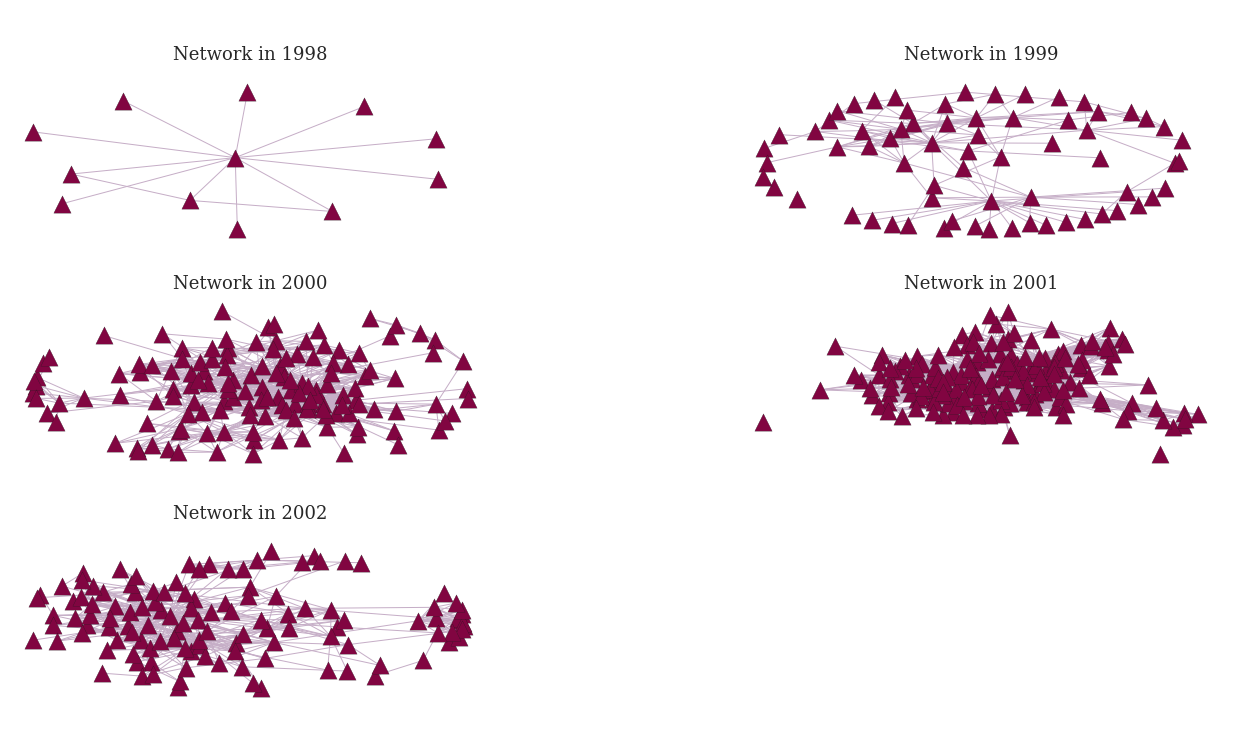
\includegraphics[height =0.7\textheight, width= 0.9\textwidth]{yearly_net.png}
    \caption{Node Link Diagram of yearly networks}
    \label{fig:Node Link Diagram for the yearly networks}
\end{figure}

\begin{figure}[H]
    \centering
    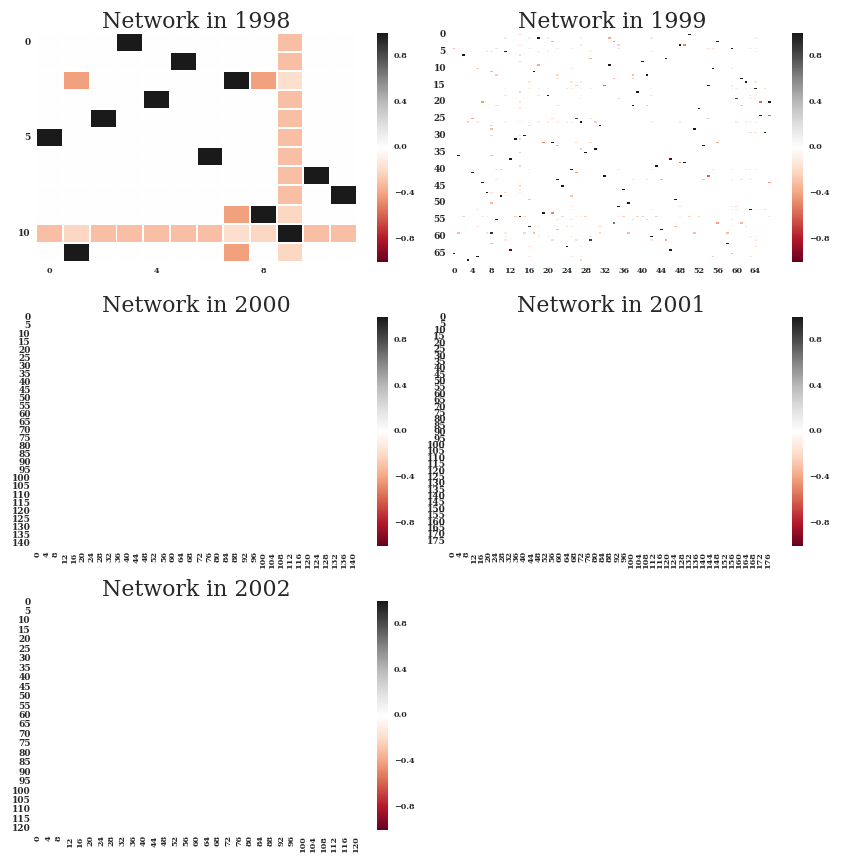
\includegraphics[height =0.9\textheight, width= 0.9\textwidth]{yearly_net_mat.png}
    \caption{Reordered Matrix Diagram of yearly networks}
    \label{fig:Reordered Matrix Diagram for the yearly networks}
\end{figure}

\begin{figure}[H]
    \centering
    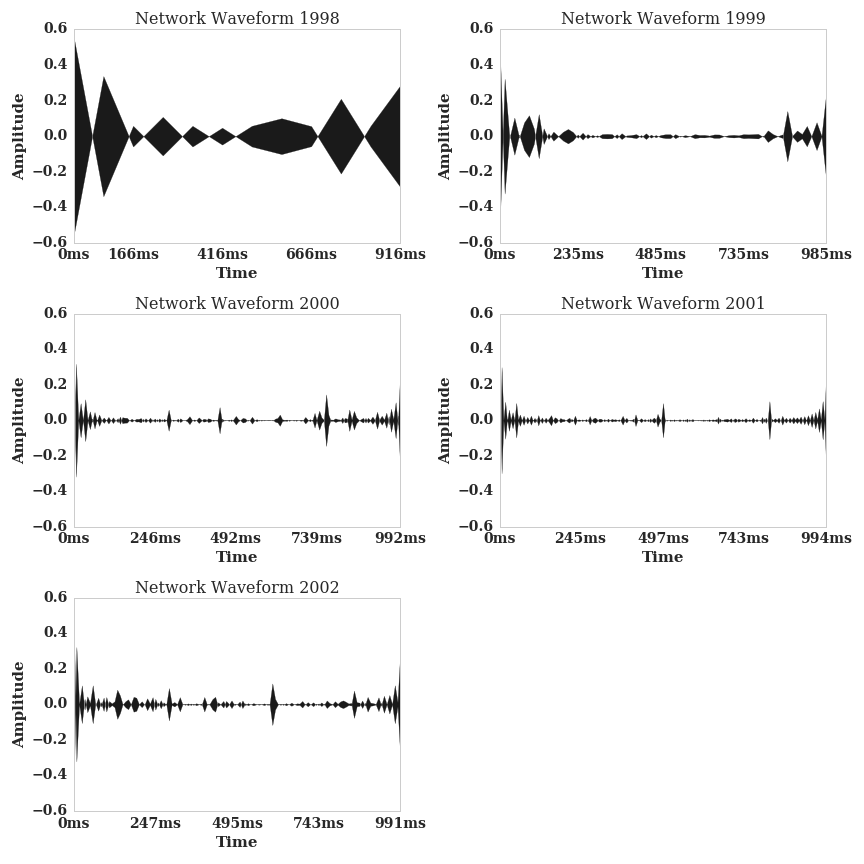
\includegraphics[height =0.9\textheight, width= 0.9\textwidth]{yearly_net_audio.png}
    \caption{Audio Waveform plot of yearly networks}
    \label{fig:Audio Waveform Plot for the yearly networks}
\end{figure}

\subsection{Monthly Network Visualisations}
\begin{figure}[H]
    \centering
    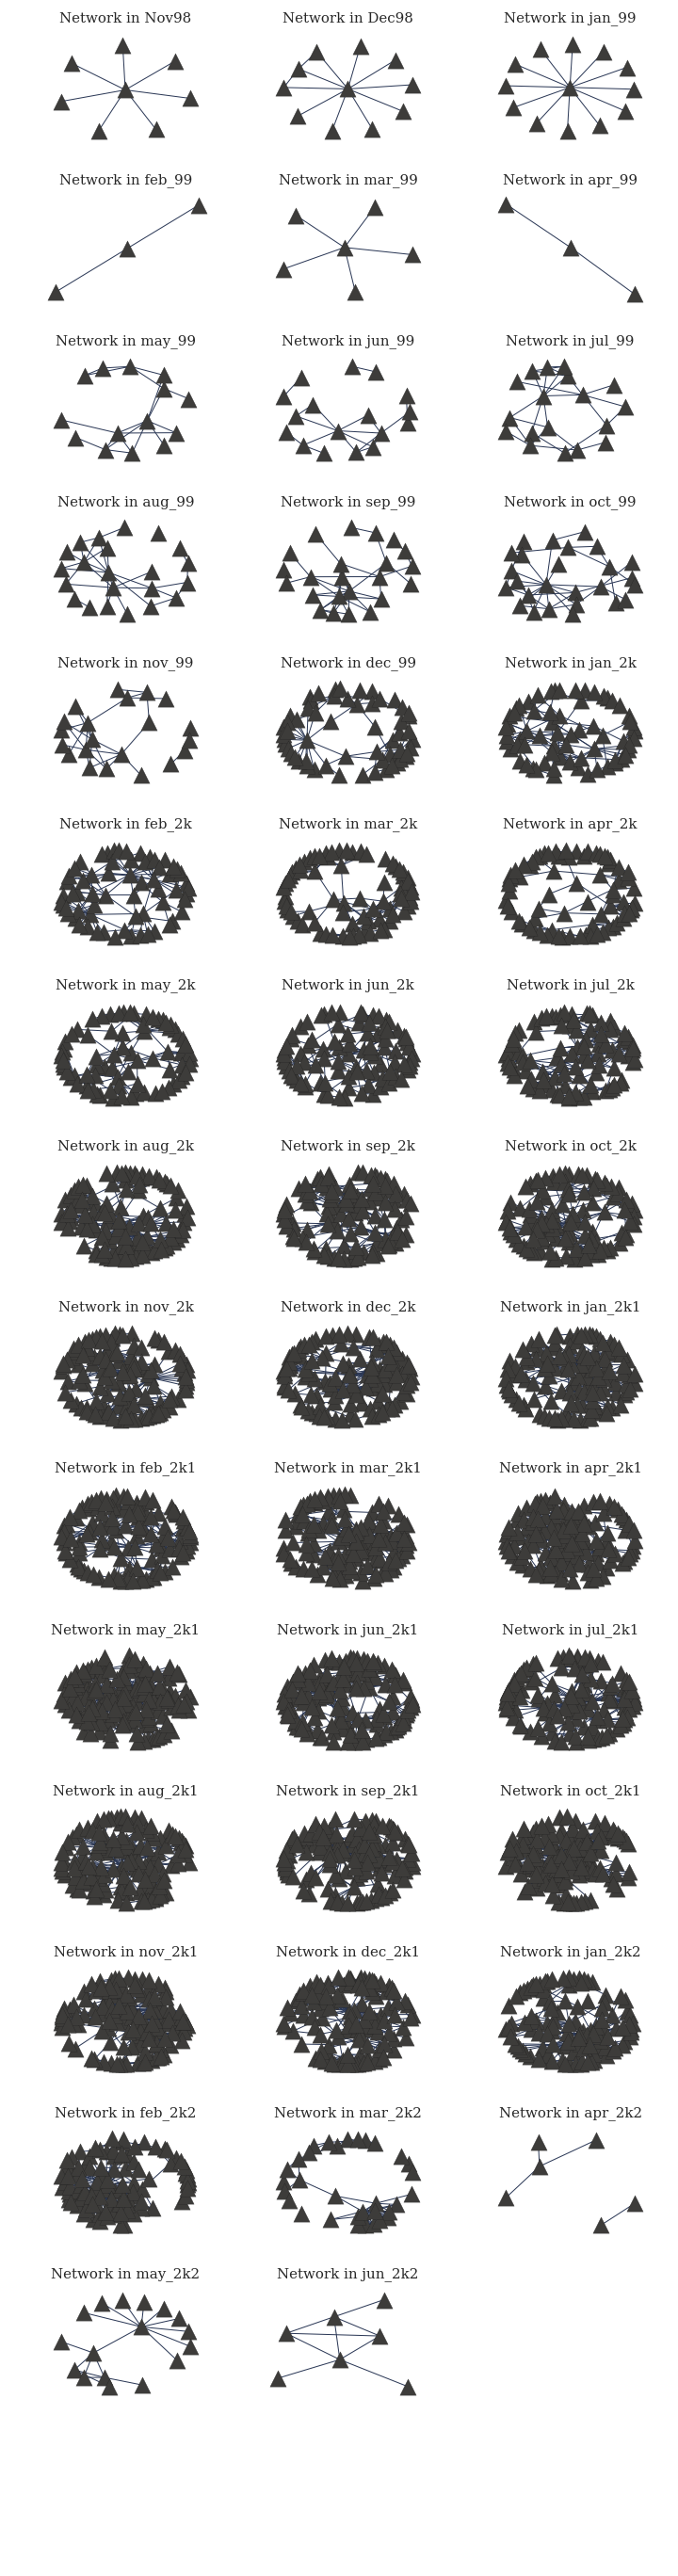
\includegraphics[height =0.9\textheight, width= 0.9\textwidth]{mth_net_nodelink.png}
    \caption{Node Link Diagram of monthly networks}
    \label{fig:node mth}
\end{figure}

\begin{figure}[H]
    \centering
    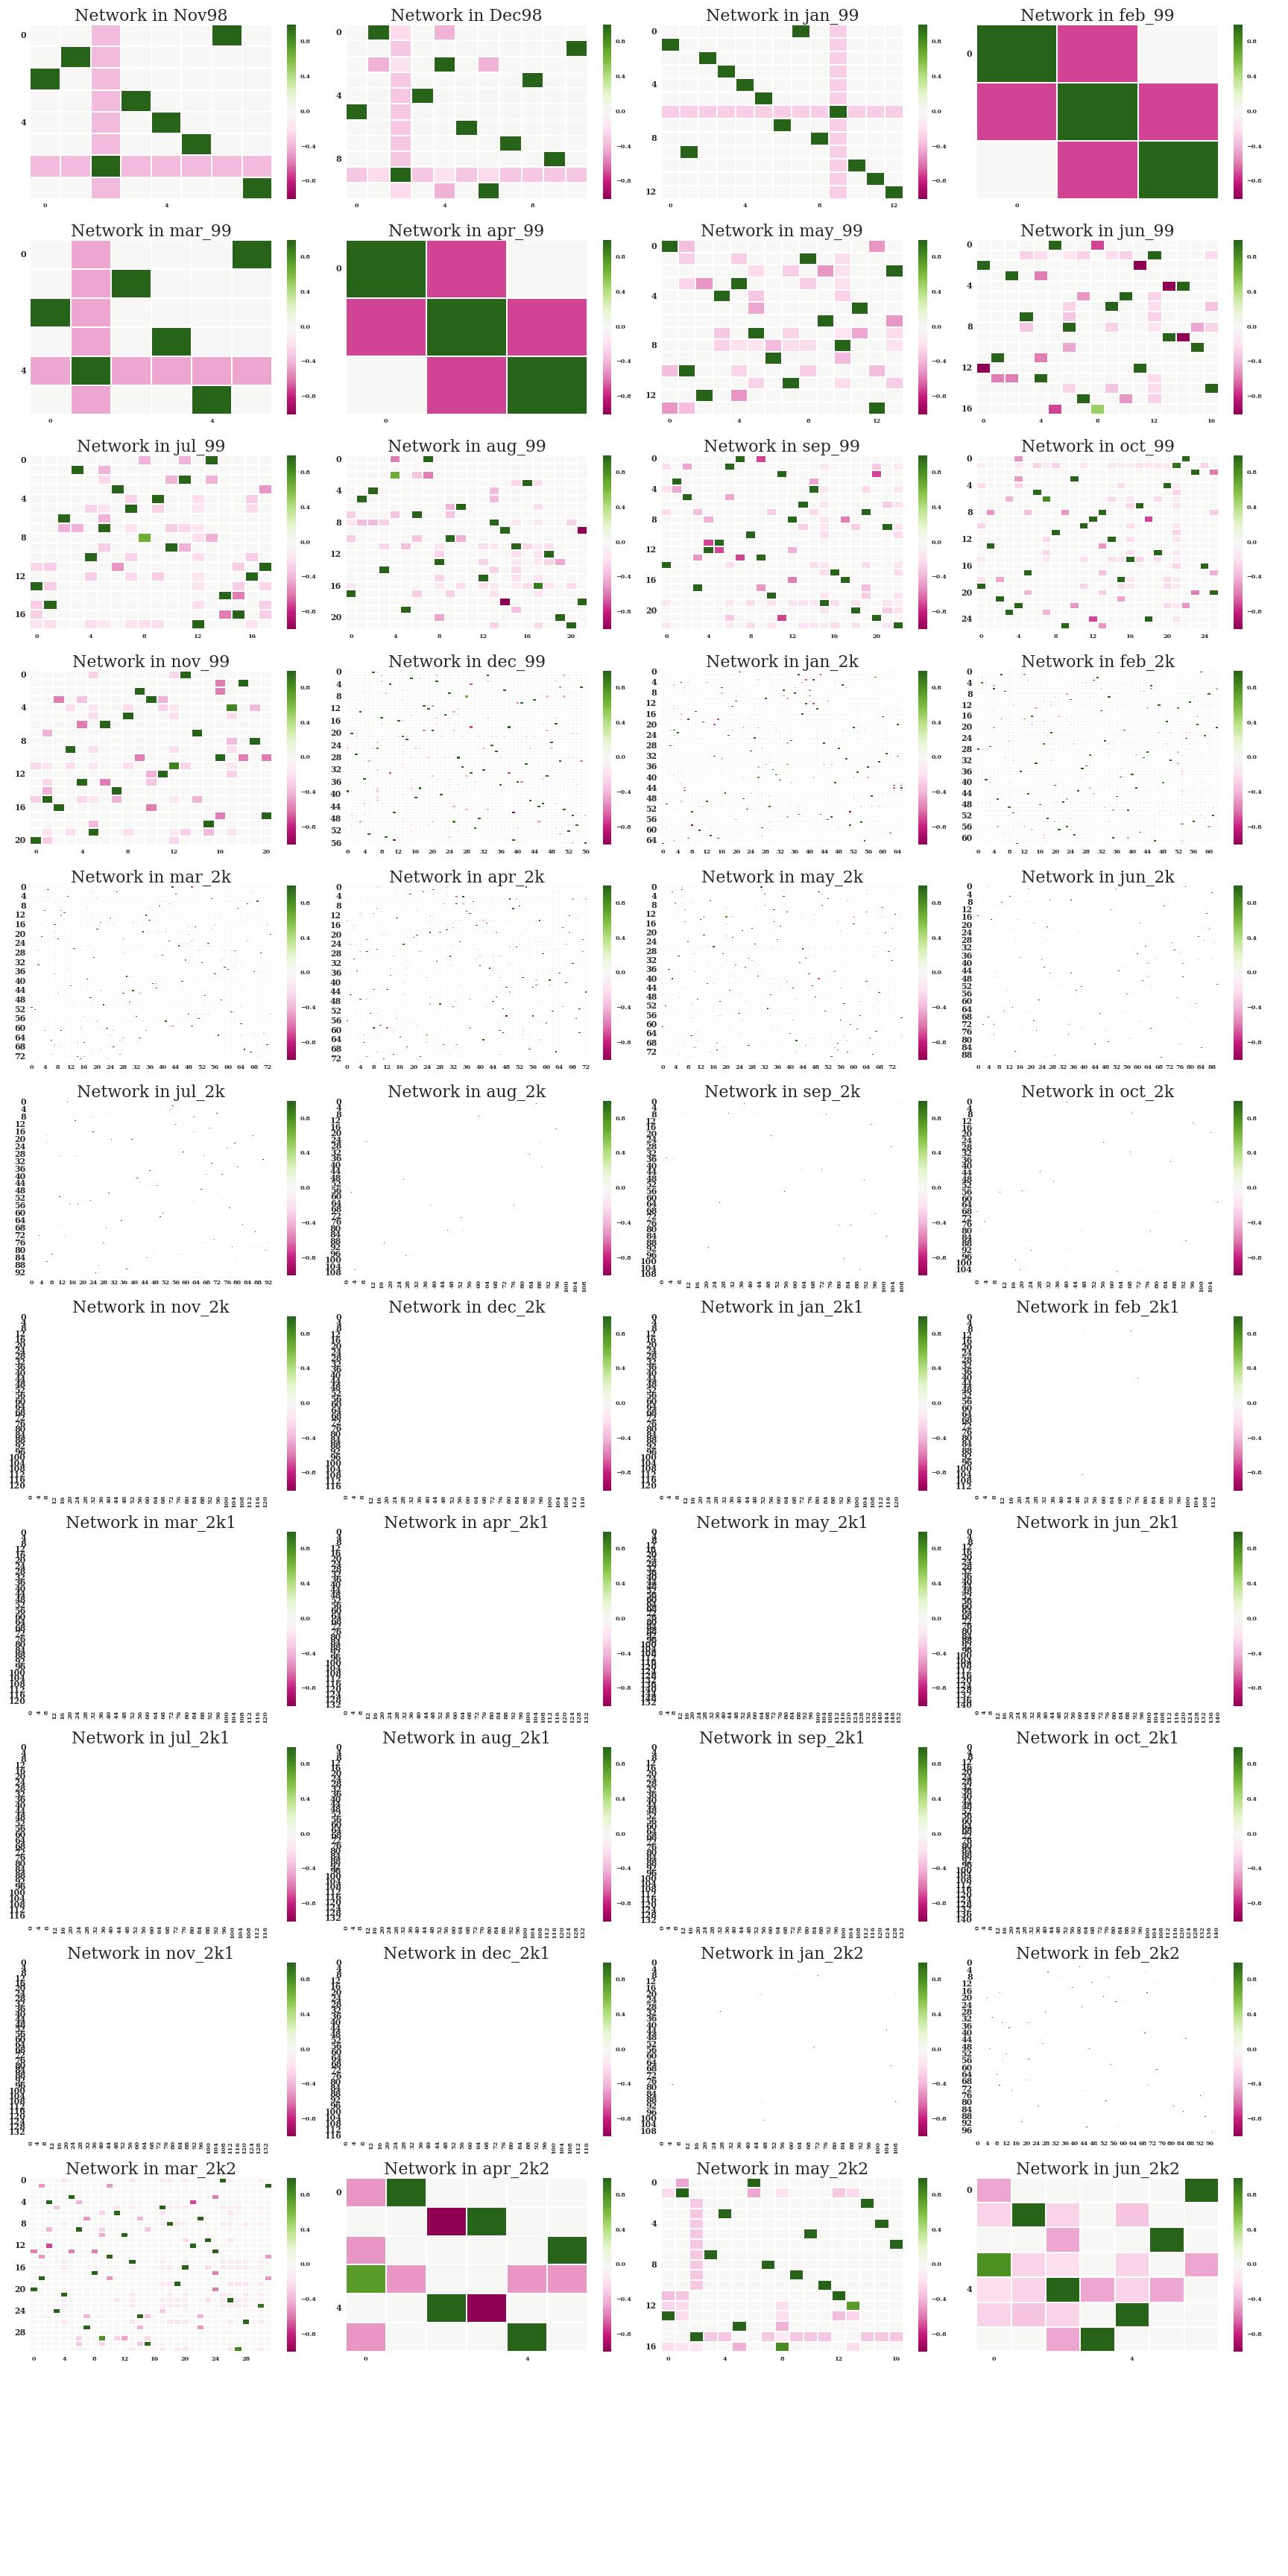
\includegraphics[height =0.9\textheight, width= 0.9\textwidth]{mth_net_mat.png}
    \caption{Reordered Matrix of monthly networks}
    \label{fig:Reordered Matrix Diagram for the monthly networks}
\end{figure}

\begin{figure}[H]
    \centering
    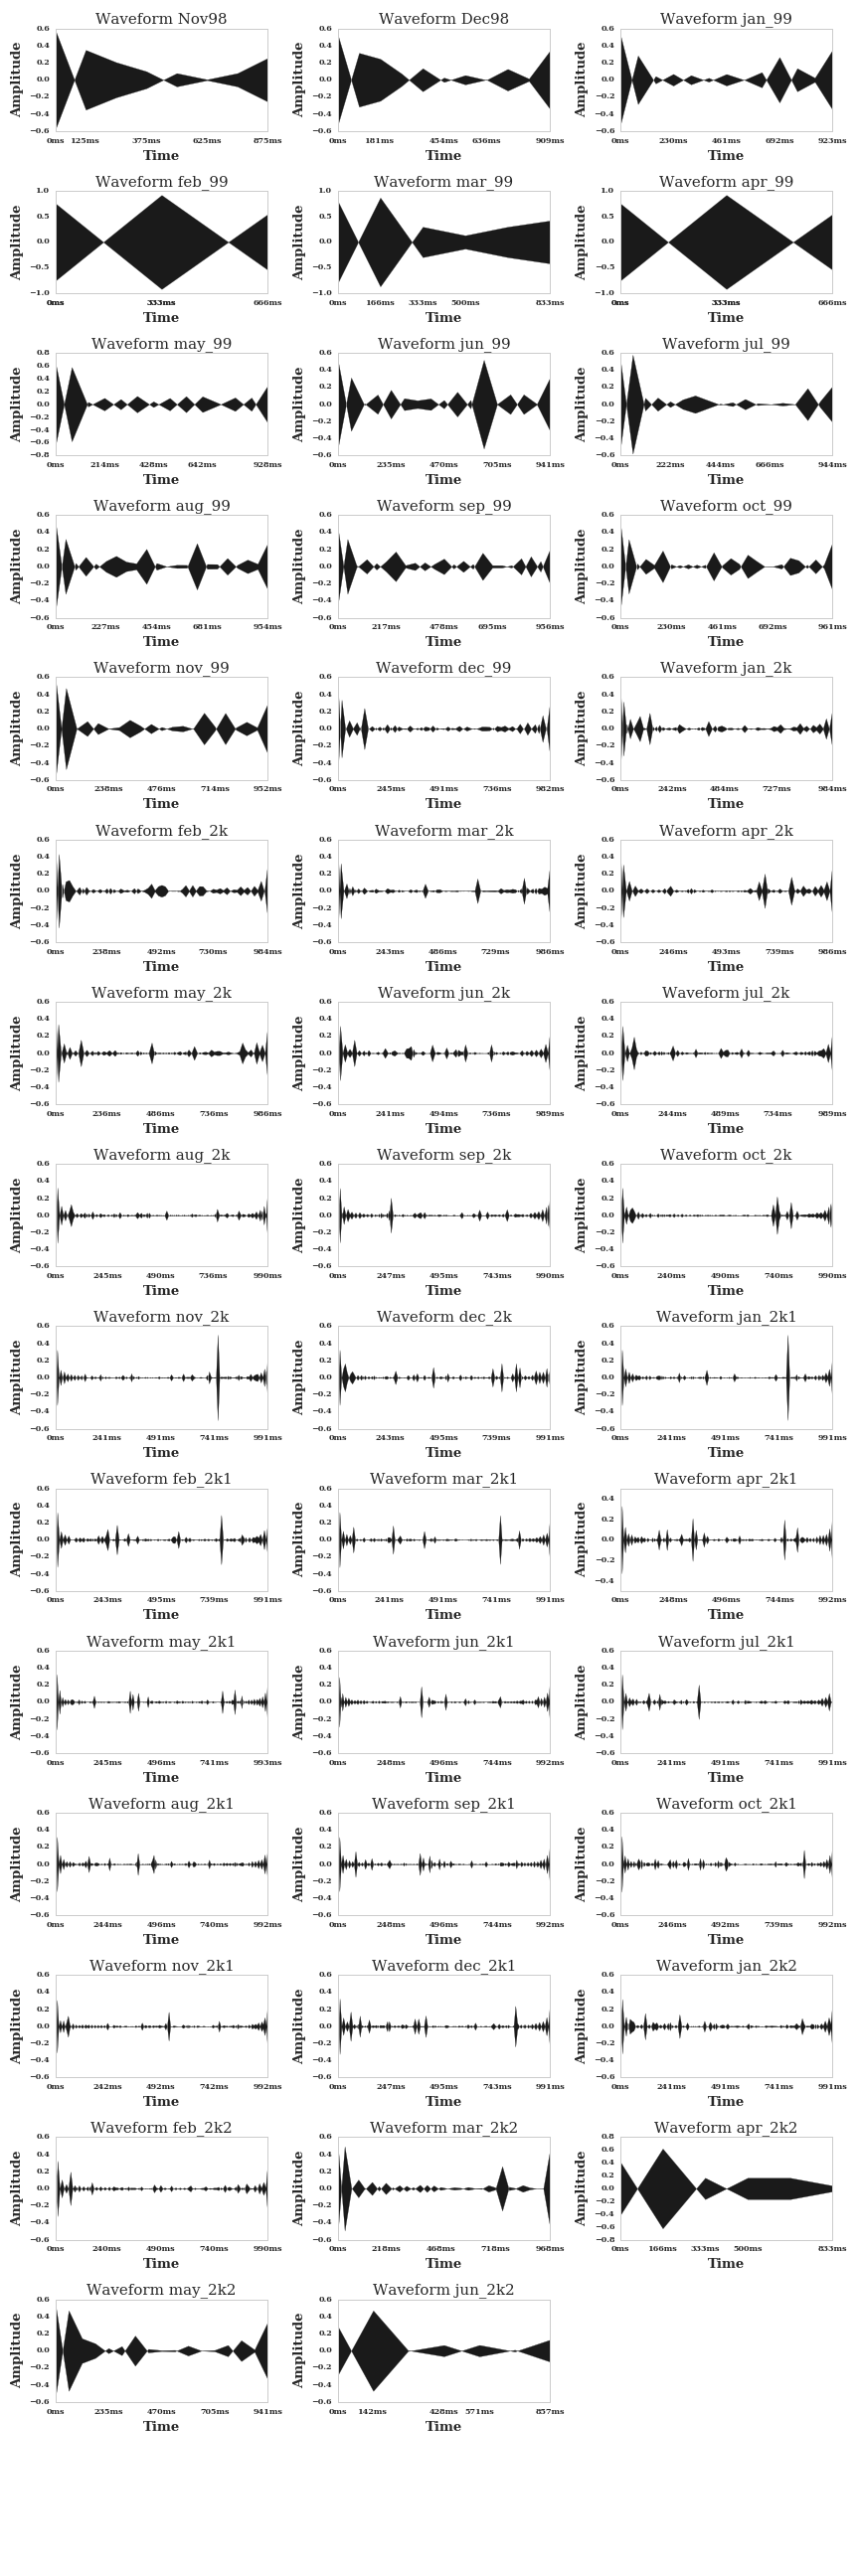
\includegraphics[height =0.9\textheight, width= 0.9\textwidth]{mth_net_audio.png}
    \caption{Audio Wavefrom  of monthly networks}
    \label{fig:Audio Waveform Plot for the monthly networks}
\end{figure}

\section{Exploratory Analysis: Centrality Measures} \label{explanal}

\subsection{Yearly Analysis}
\begin{figure}[H]
    \centering
    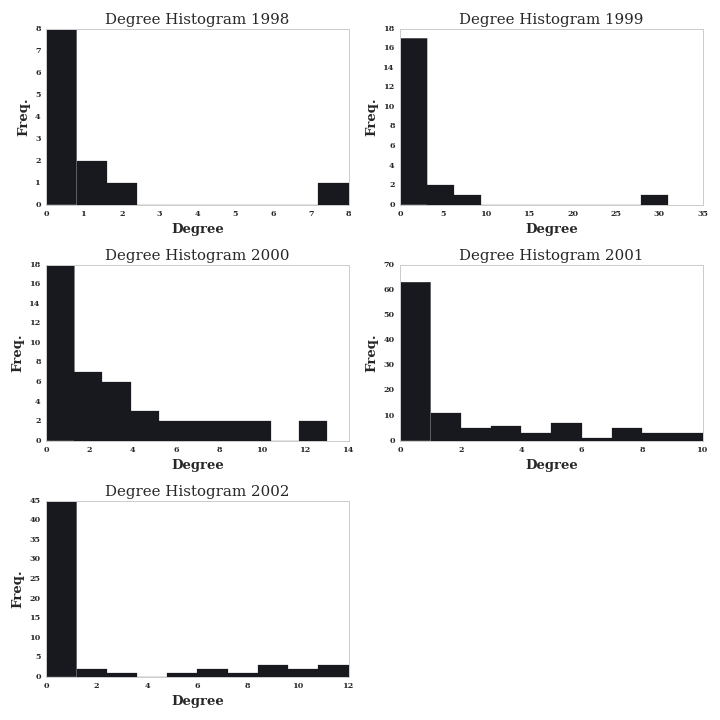
\includegraphics[height =0.9\textheight, width= 0.9\textwidth]{year_deghist.png}
    \caption{Yearly Degree Histogram}
    \label{fig:Yearly Degree Histogram}
\end{figure}

\begin{figure}[H]
    \centering
    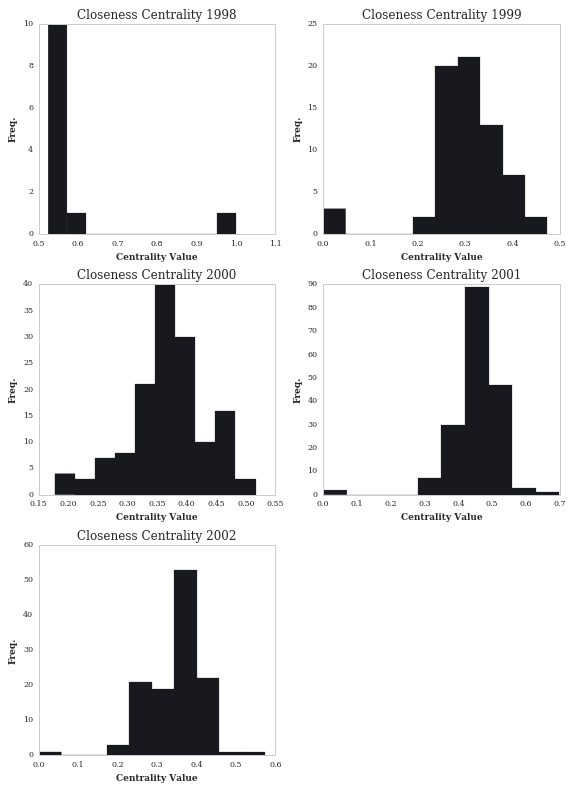
\includegraphics[height =0.9\textheight, width= 0.9\textwidth]{year_clohist.png}
    \caption{Yearly Closeness Centrality Histogram}
    \label{fig:Yearly Closeness Centrality Histogram}
\end{figure}

\begin{figure}[H]
    \centering
    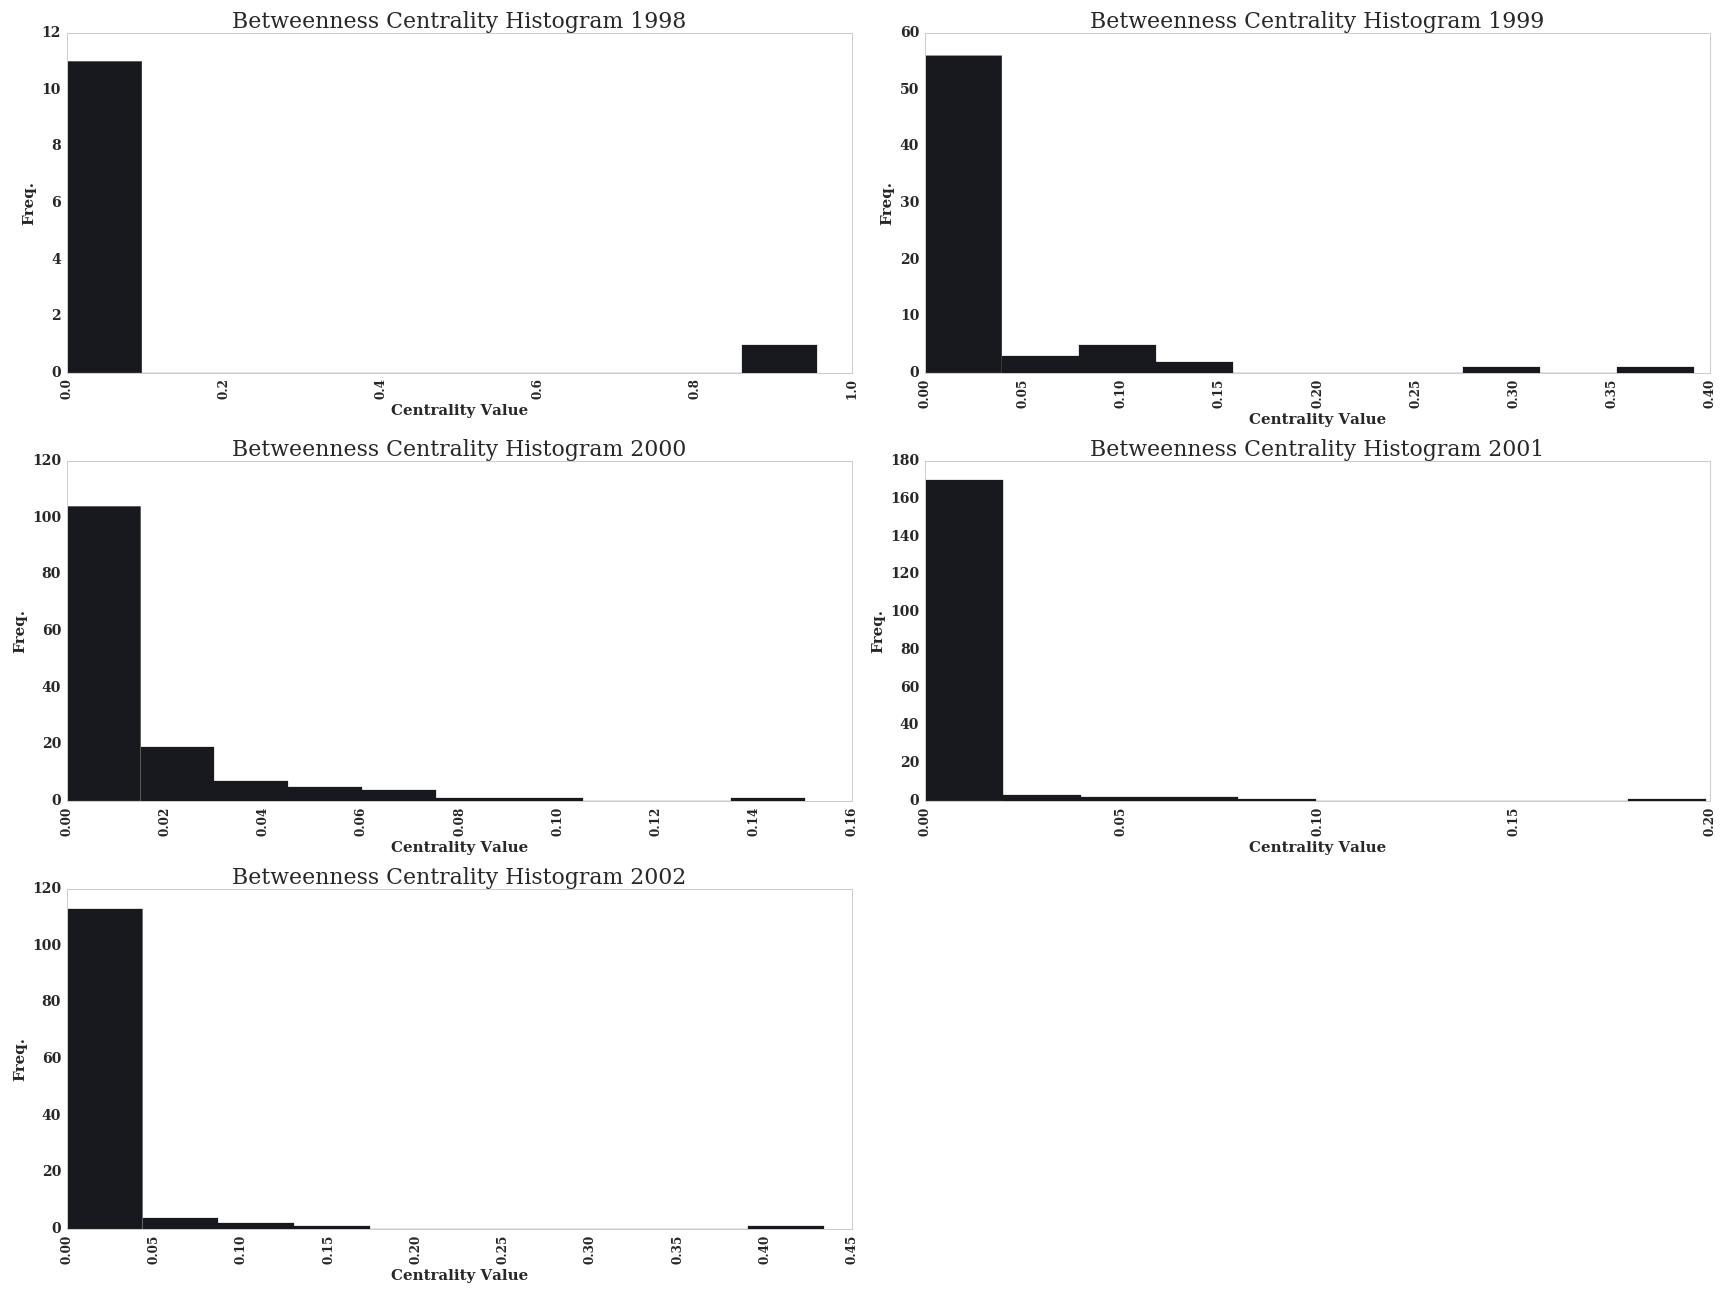
\includegraphics[height =0.9\textheight, width= 0.9\textwidth]{year_bethist.png}
    \caption{Yearly Betweenness Histogram}
    \label{fig:Yearly Betweenness Centrality Histogram}
\end{figure}

\begin{figure}[H]
    \centering
    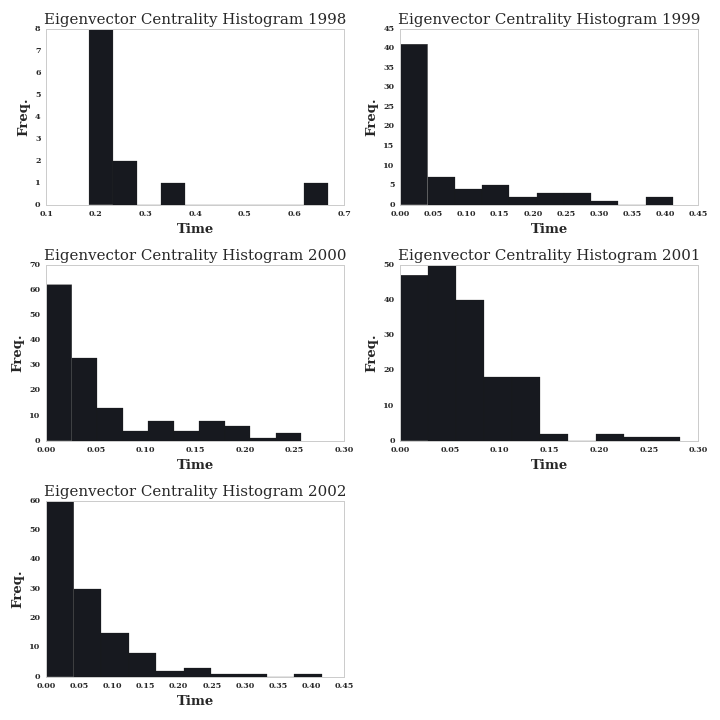
\includegraphics[height =0.9\textheight, width= 0.9\textwidth]{year_eighist.png}
    \caption{Yearly Eigenvector Centrality Histogram}
    \label{fig:Yearly Eigenvector Centrality Histogram}
\end{figure}

\begin{figure}[H]
    \centering
    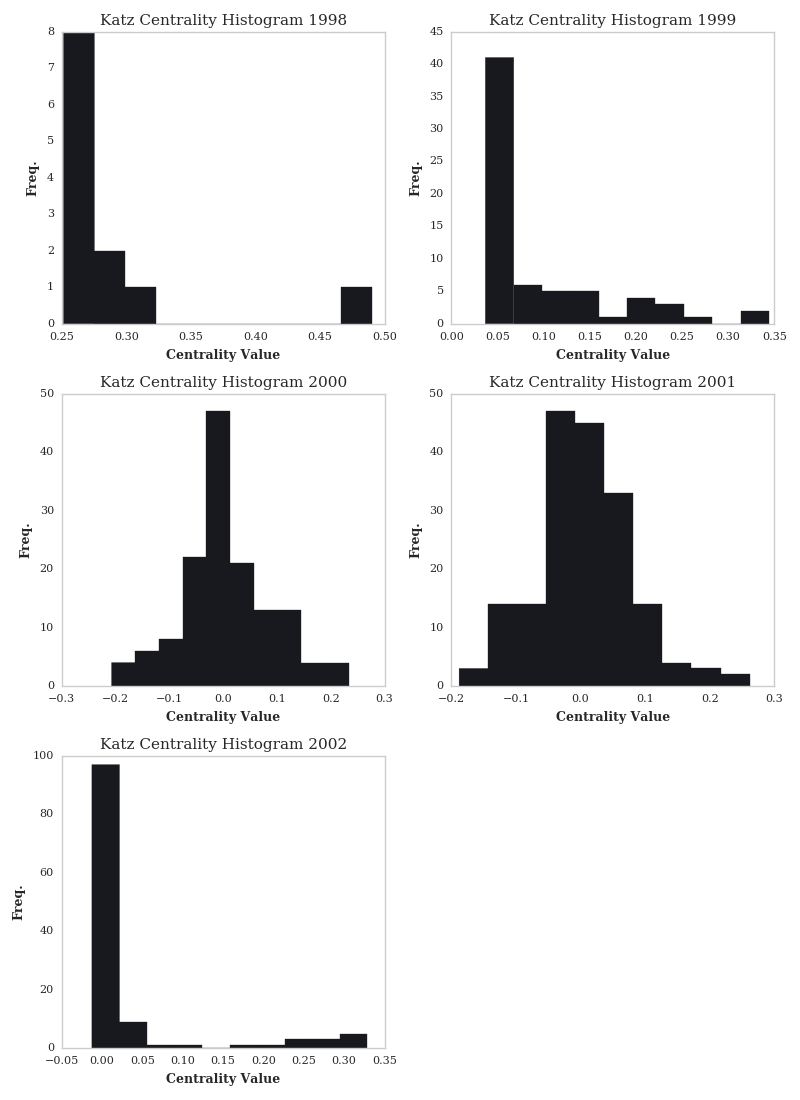
\includegraphics[height =0.9\textheight, width= 0.9\textwidth]{year_katzhist.png}
    \caption{Yearly Katz Centrality Histogram}
    \label{fig:Yearly Katz Centrality Histogram}
\end{figure}

\begin{figure}[H]
    \centering
    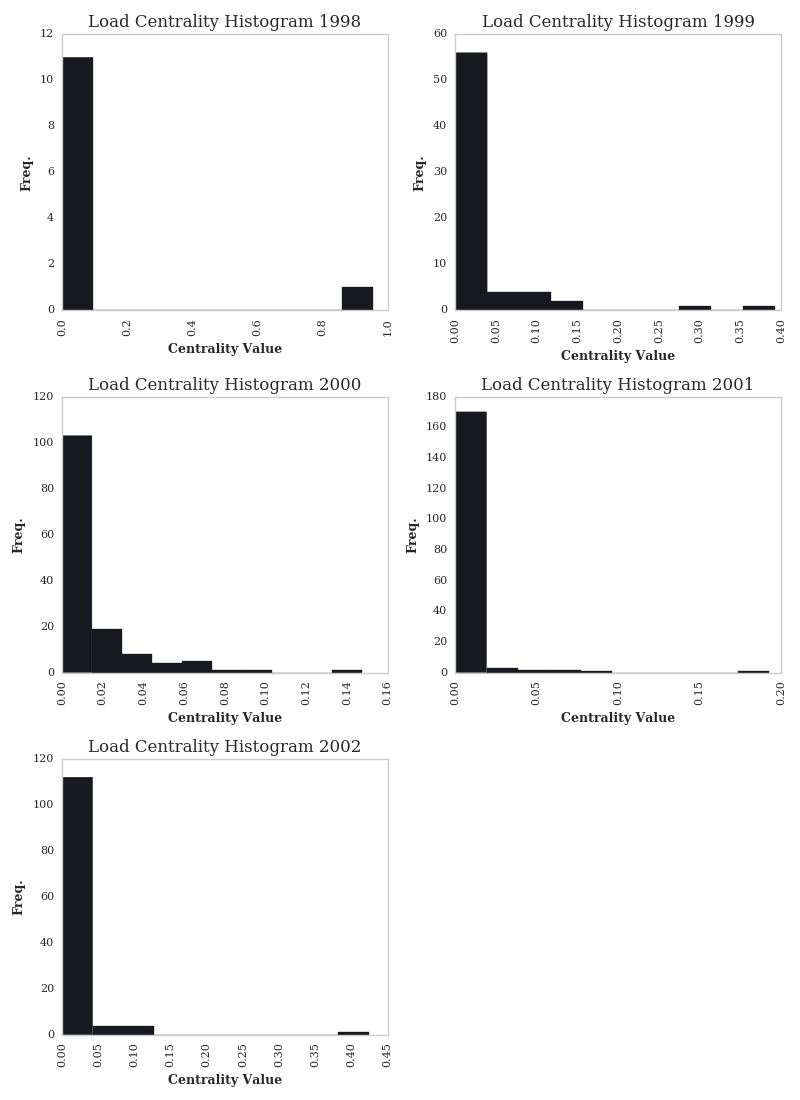
\includegraphics[height =0.9\textheight, width= 0.9\textwidth]{year_loadhist.png}
    \caption{Yearly Load Centrality Histogram}
    \label{fig:Yearly Load Centrality Histogram}
\end{figure}

\subsection{Monthly Analysis}
\begin{figure}[H]
    \centering
    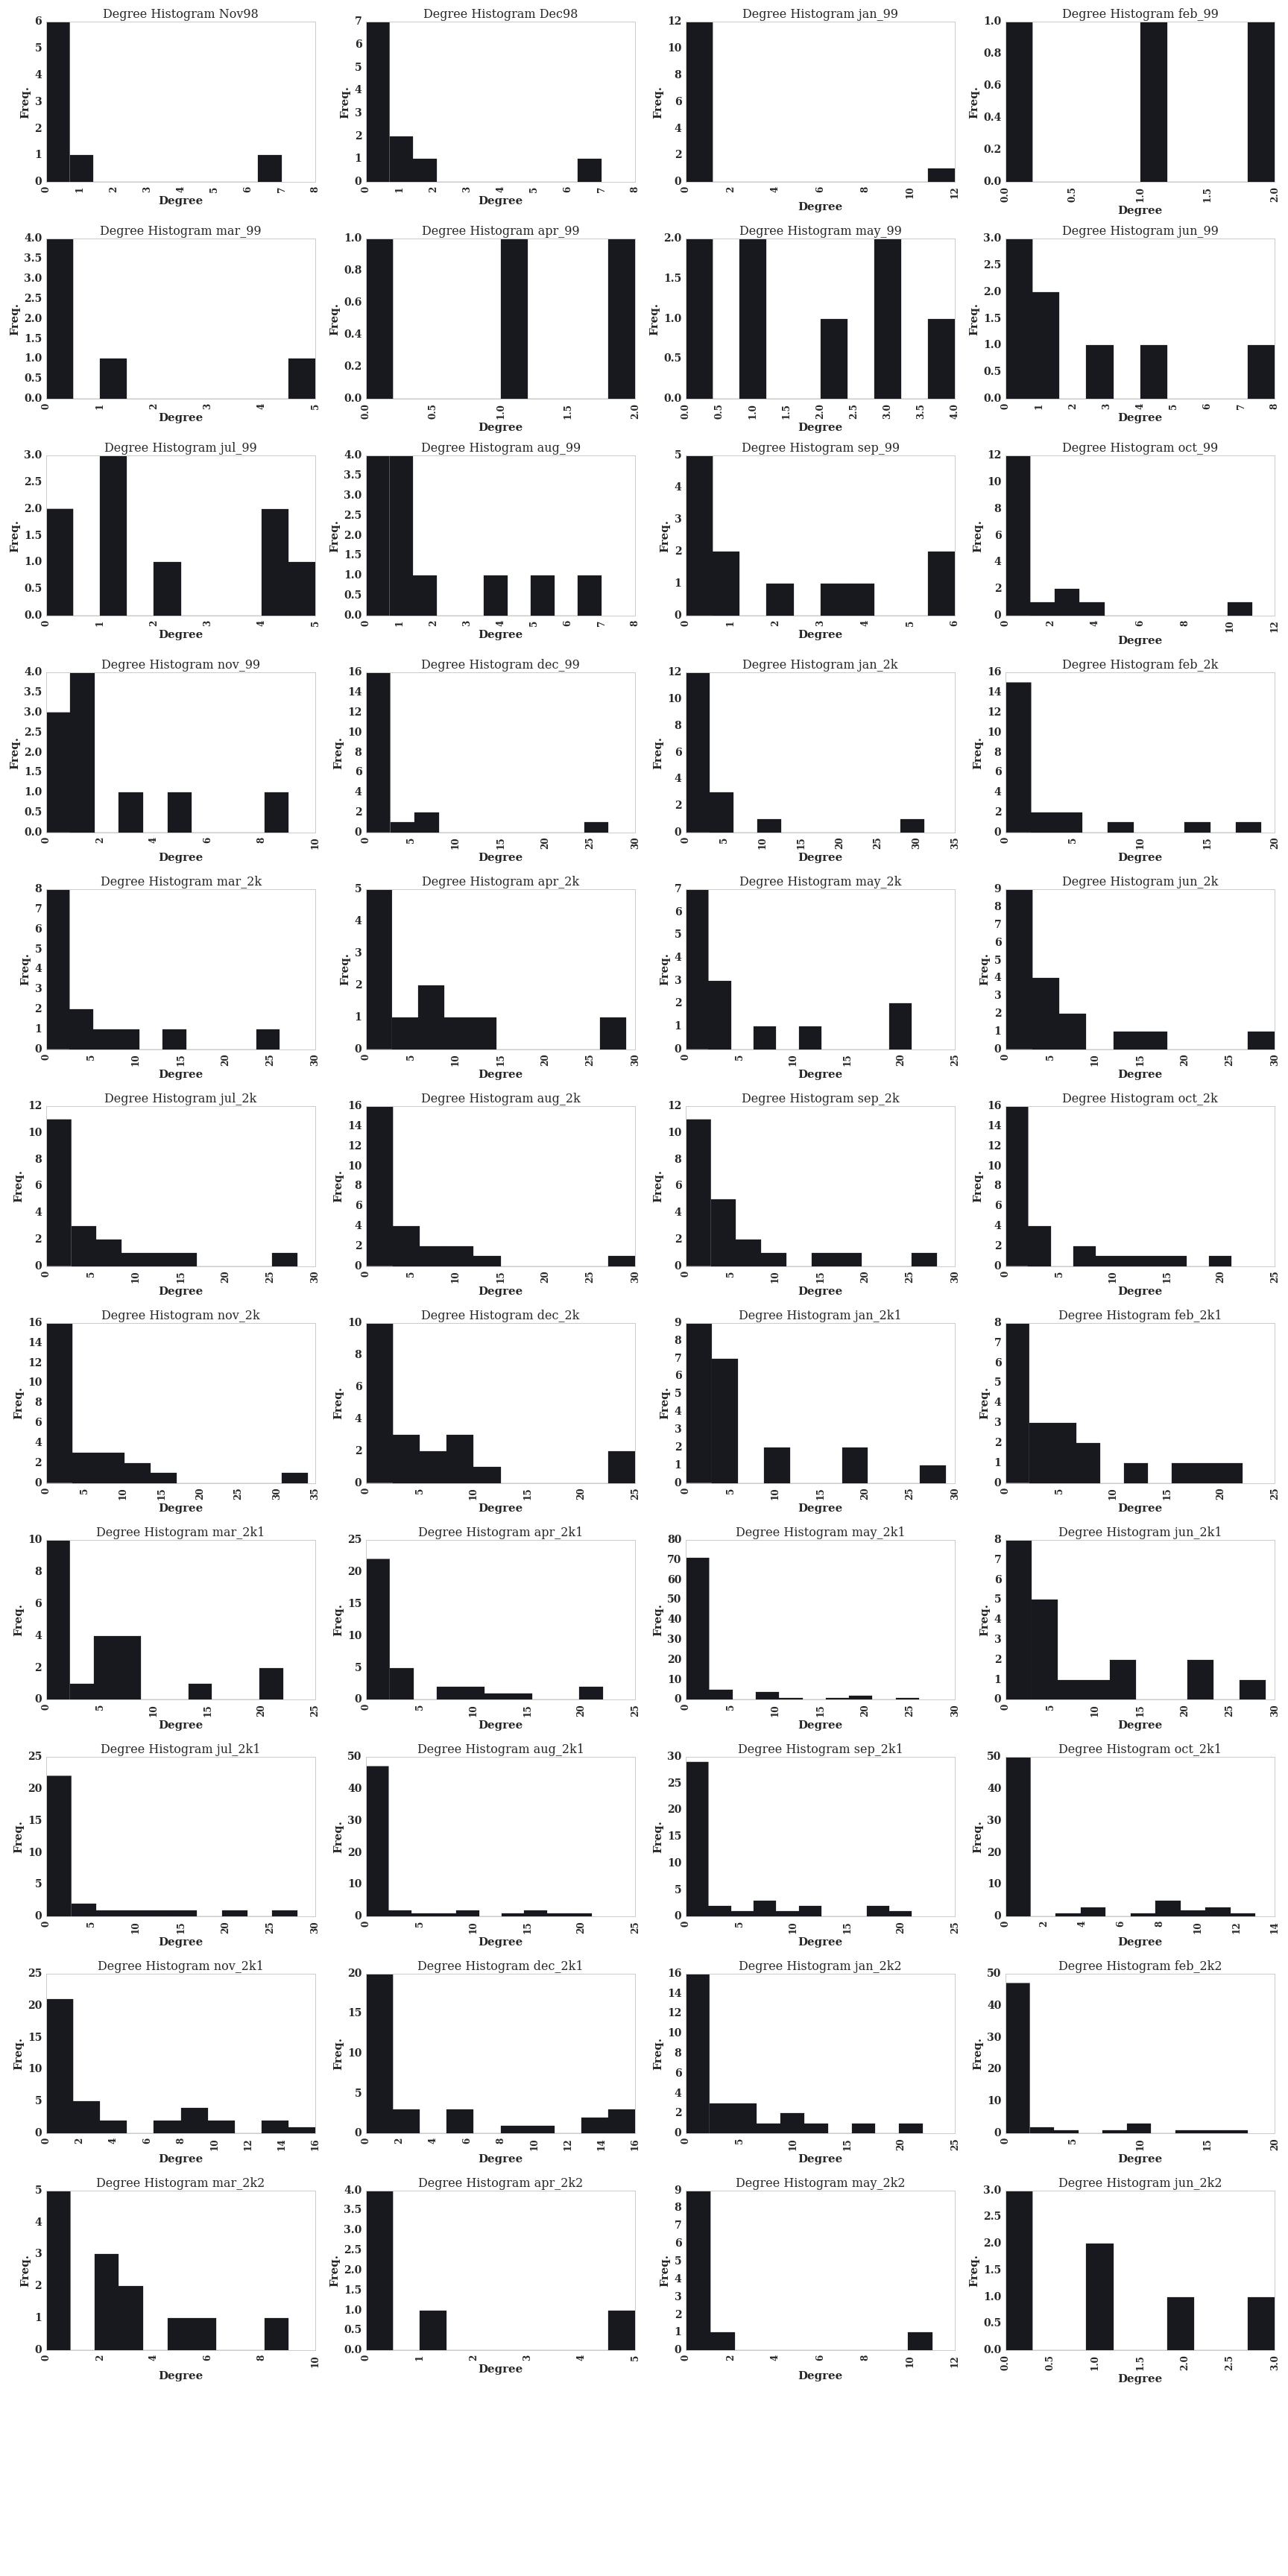
\includegraphics[height =0.9\textheight, width= 0.9\textwidth]{mth_deghist.png}
    \caption{Monthly Degree Histogram}
    \label{fig:Monthly Degree Histogram}
\end{figure}

\begin{figure}[H]
    \centering
    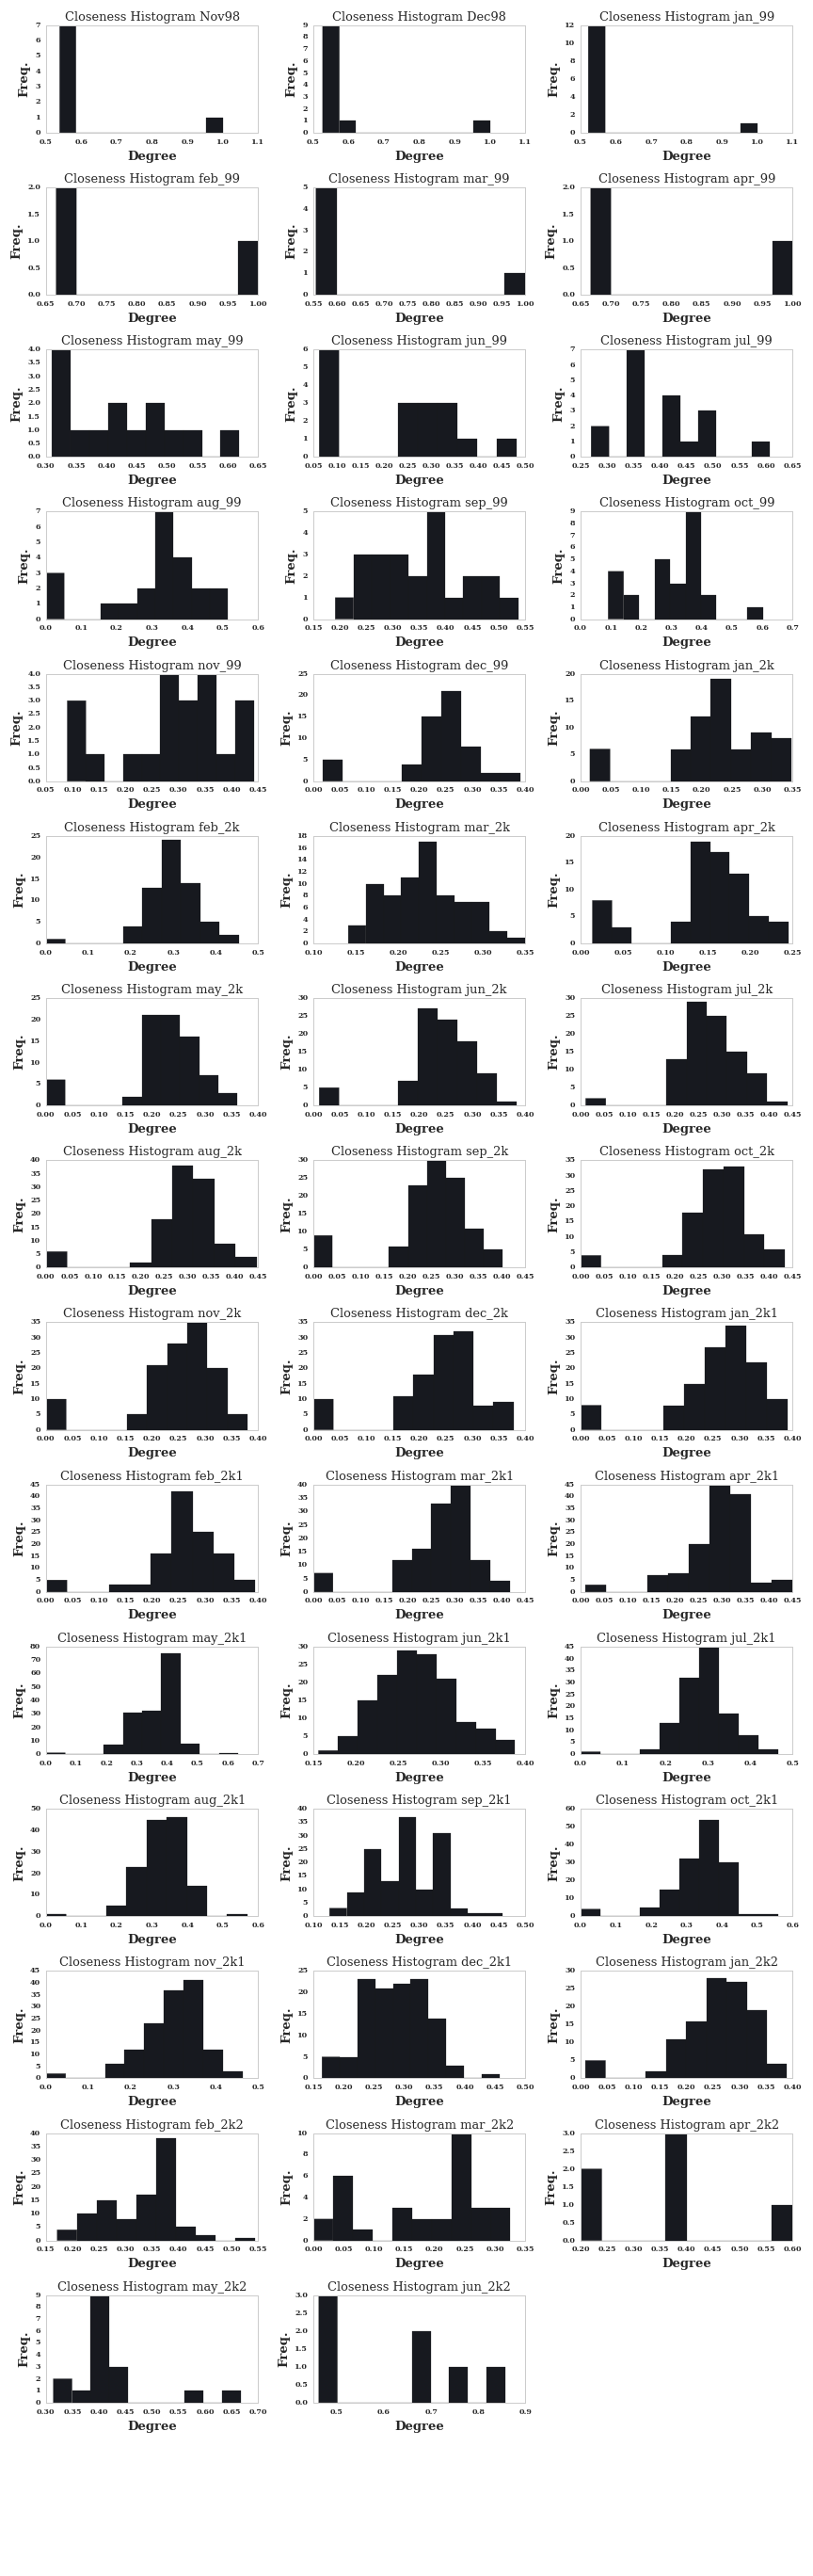
\includegraphics[height =0.9\textheight, width= 0.9\textwidth]{mth_clohist.png}
    \caption{Monthly Closeness Centrality Histogram}
    \label{fig:Monthly Closeness Centrality Histogram}
\end{figure}

\begin{figure}[H]
    \centering
    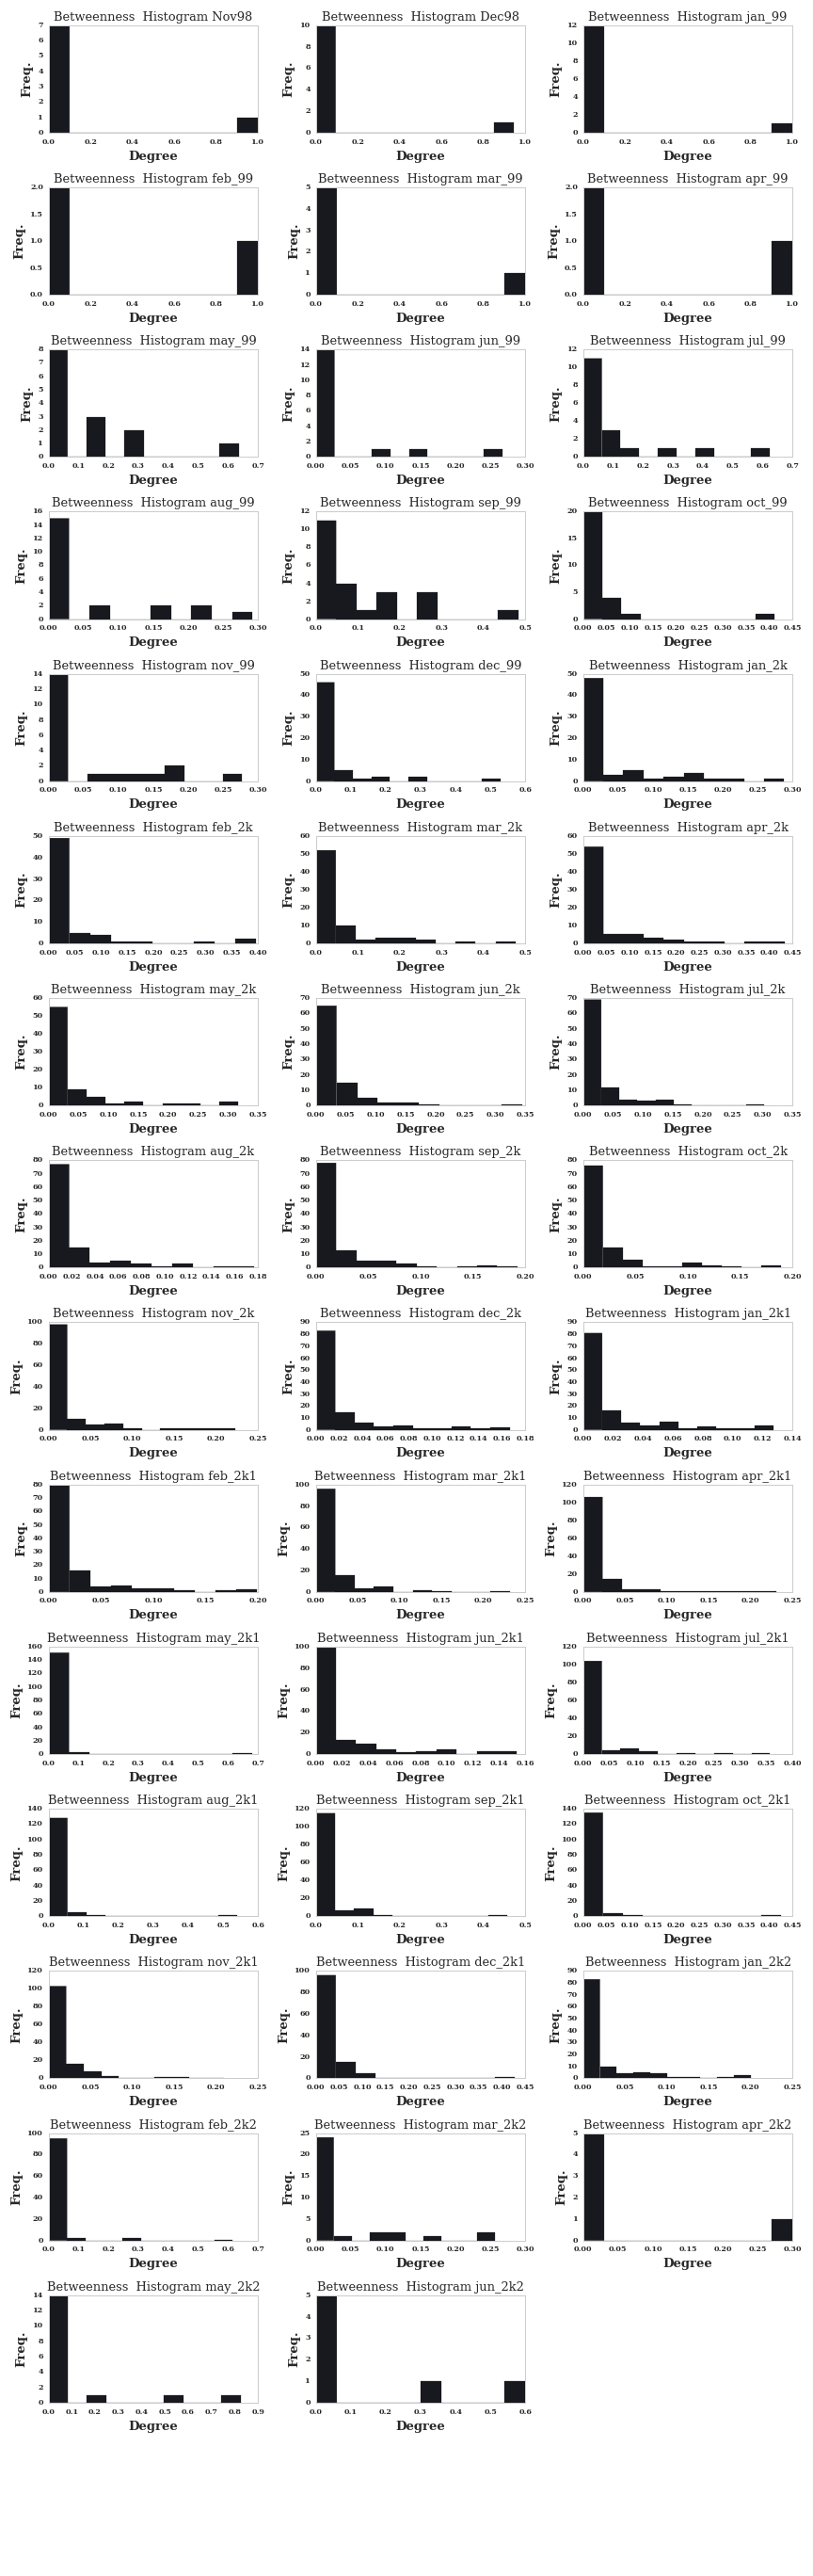
\includegraphics[height =0.9\textheight, width= 0.9\textwidth]{mth_bethist.png}
    \caption{Monthly Betweenness Histogram}
    \label{fig:Monthly Betweenness Centrality Histogram}
\end{figure}

\begin{figure}[H]
    \centering
    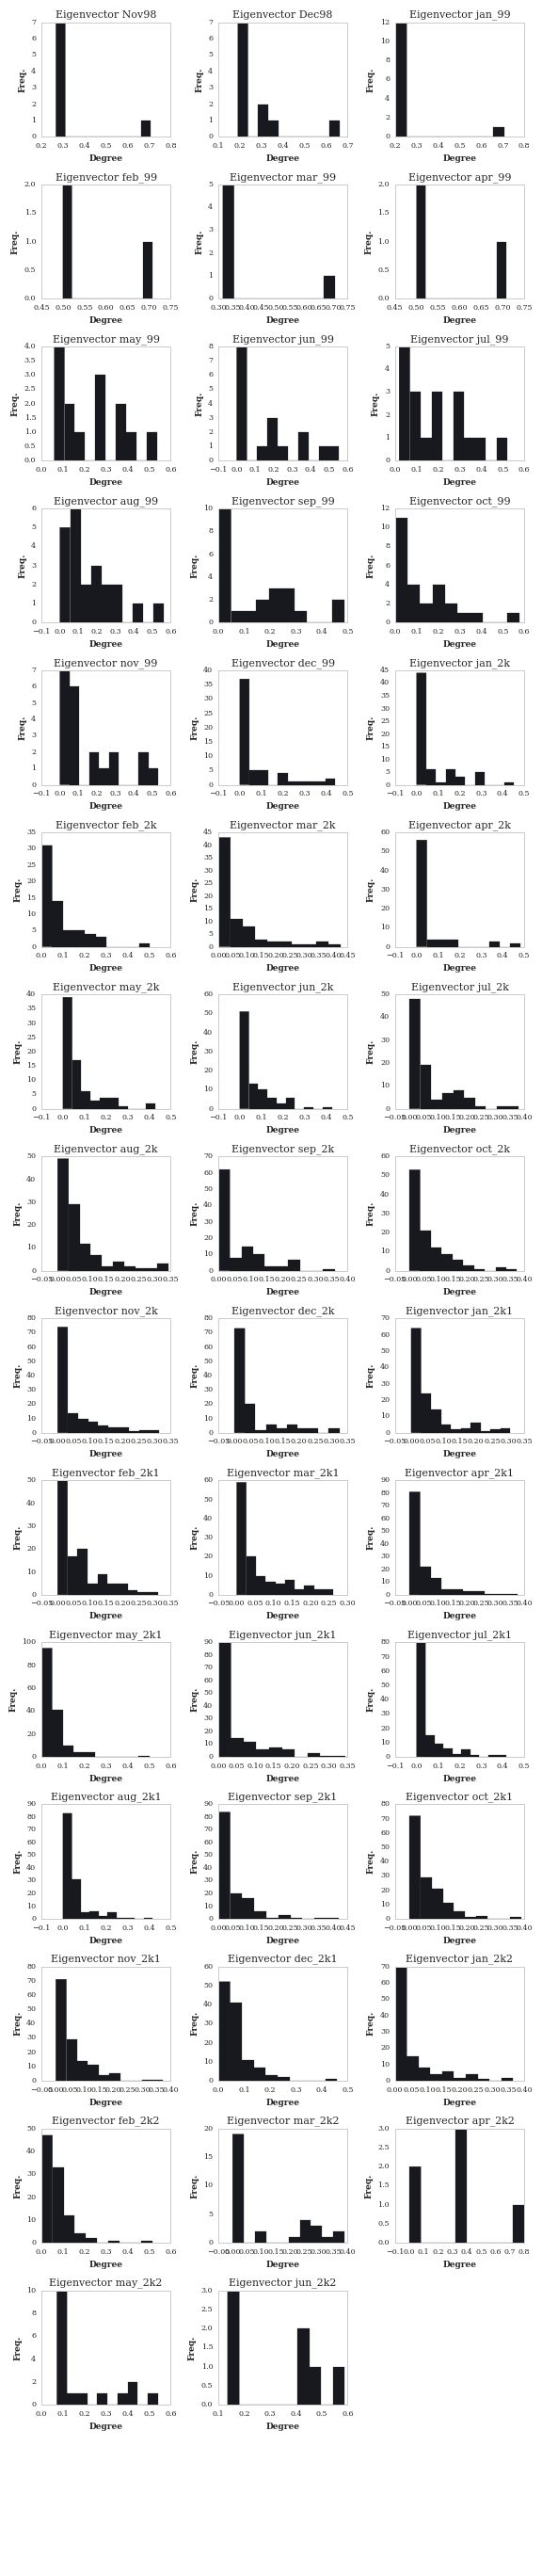
\includegraphics[height =0.9\textheight, width= 0.9\textwidth]{mth_eighist.png}
    \caption{Monthly Eigenvector Centrality Histogram}
    \label{fig:Monthly Eigenvector Centrality Histogram}
\end{figure}

\begin{figure}[H]
    \centering
    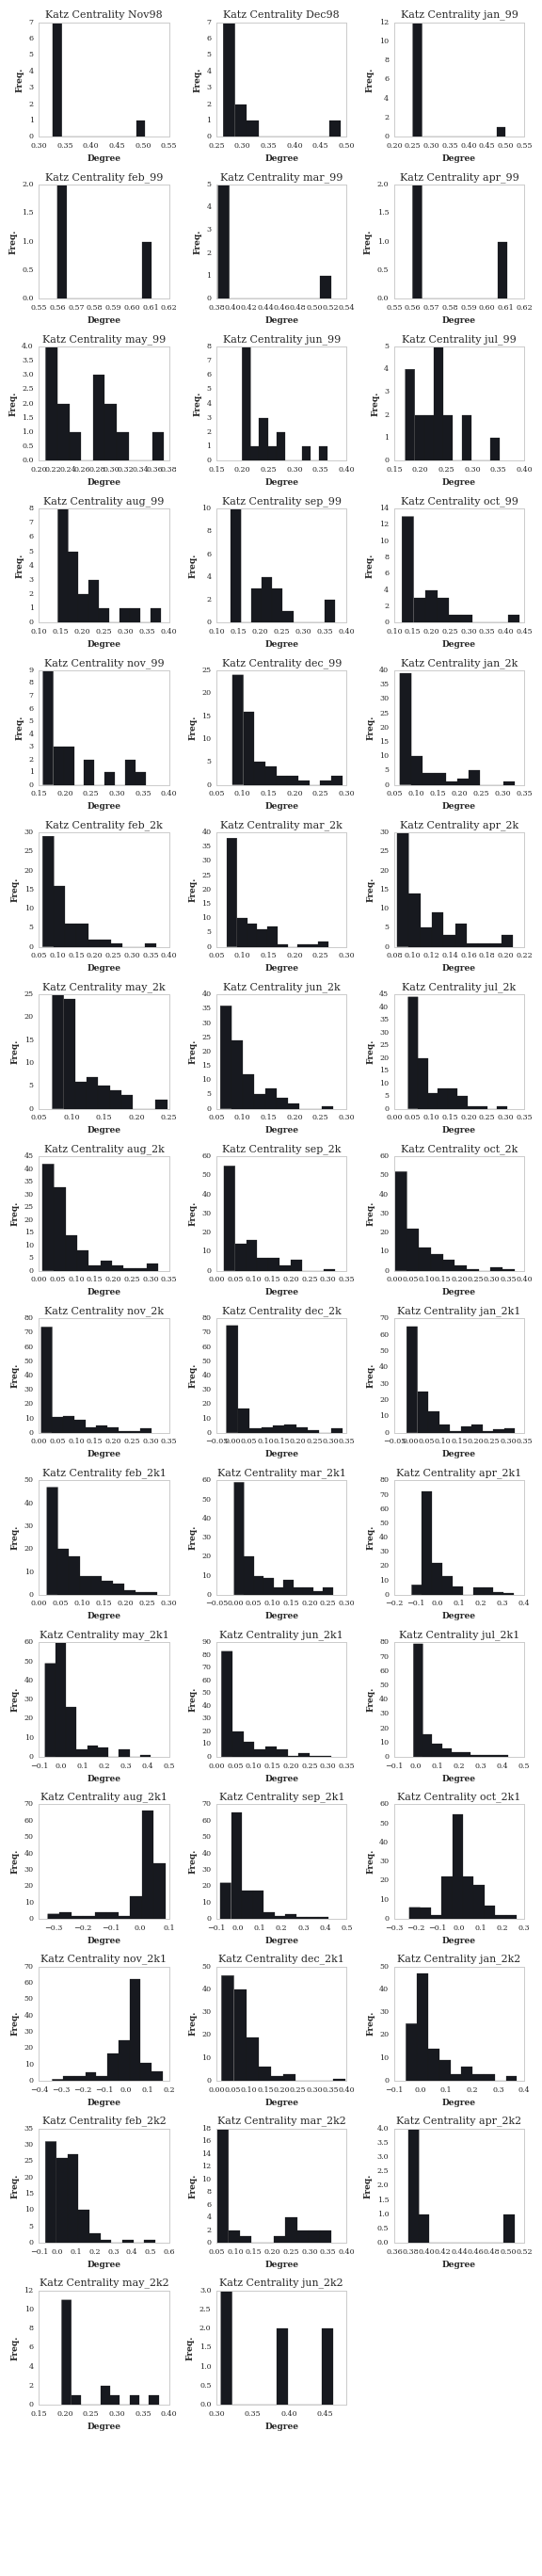
\includegraphics[height =0.9\textheight, width= 0.9\textwidth]{mth_katzhist.png}
    \caption{Monthly Katz Centrality Histogram}
    \label{fig:Monthly Katz Centrality Histogram}
\end{figure}

\begin{figure}[H]
    \centering
    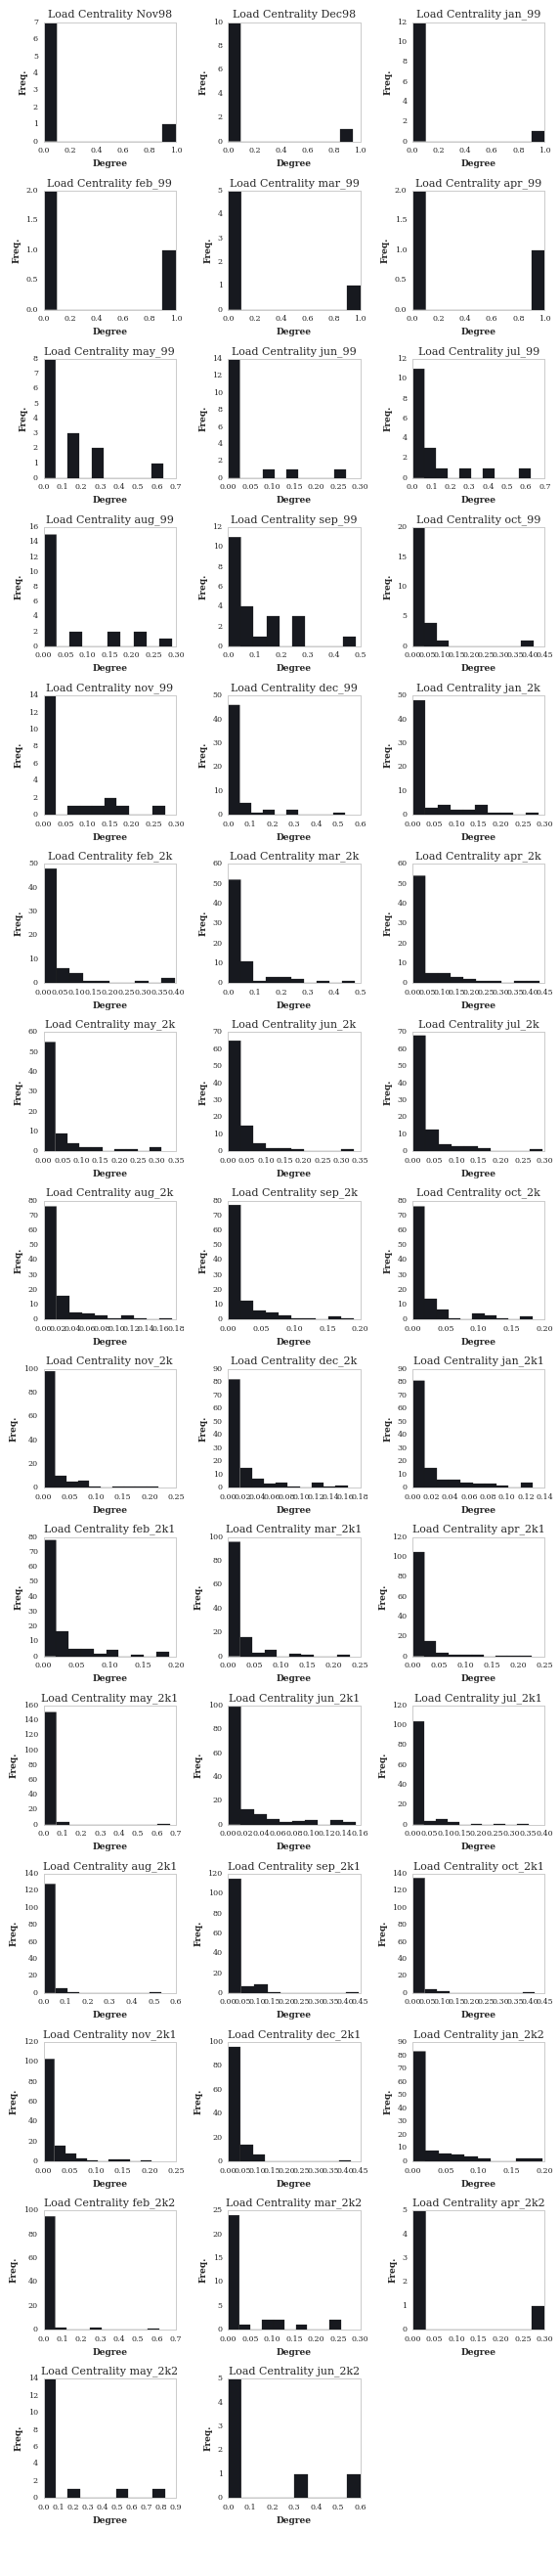
\includegraphics[height =0.9\textheight, width= 0.9\textwidth]{mth_loadhist.png}
    \caption{Monthly Load Centrality Histogram}
    \label{fig:Monthly Load Centrality Histogram}
\end{figure}

\section{Benchmark Measures}\label{bmark}

Here I plot the benchmark measures for the yearly and monthly networks to establish a signal in the graph time series. The measures proposed are judged firstly on their ability to model similar phenomenon and highlight additional interesting areas not obvious form these measures alone. \\

\begin{figure}[!htp]
    \centering
    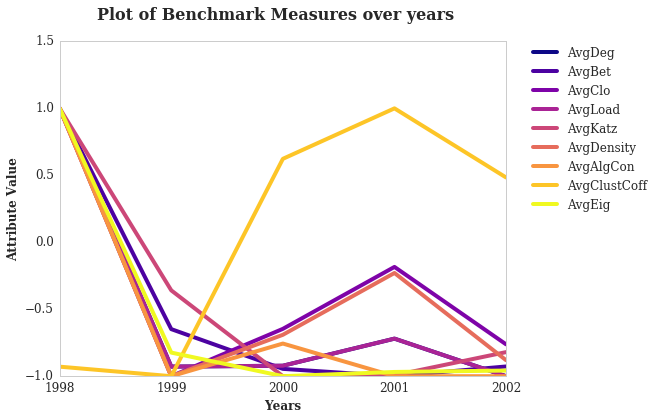
\includegraphics[height =0.3\textheight, width= 0.9\textwidth]{benchmark_yrs.png}
    \caption{Plot of Benchmark Measures over Years}
    \label{fig:bmark yrs}
\end{figure}

\begin{figure}[!htp]
    \centering
    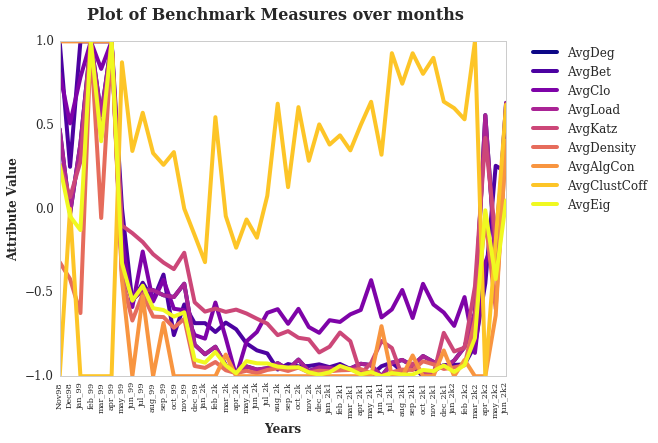
\includegraphics[height =0.3\textheight, width= 0.9\textwidth]{benchmark_mth.png}
    \caption{Plot of Benchmark Measures over Months}
    \label{fig:bmark mth}
\end{figure}

\clearpage{}
\section{Attribute Analysis}\label{attanal}

Here the novel measures proposed in this study are presented. First, I explore how the attributes vary when derived from different graph matrices.\\

\begin{figure}[!htp]
    \centering
    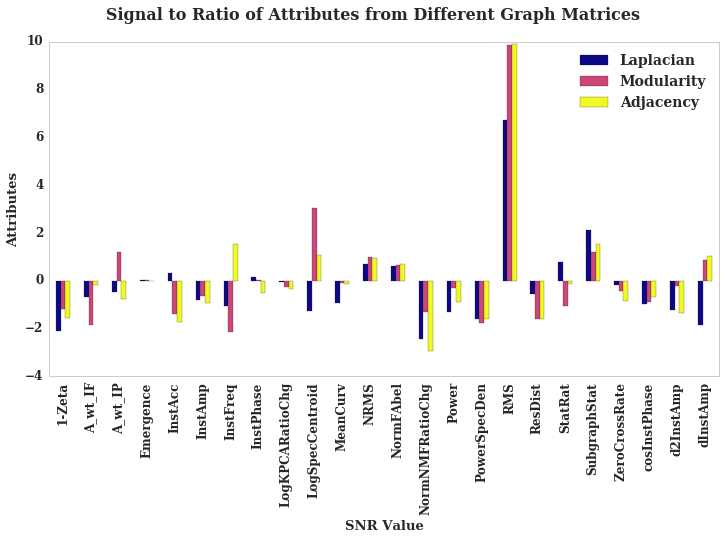
\includegraphics[height =0.4\textheight, width= 0.9\textwidth]{snr_allatt_3mat.png}
    \caption{Plot of Signal to Noise Ratio of Attributes calculated from 3 different Graph Matrices}
    \label{fig:snr}
\end{figure}

\begin{figure}[!htp]
    \centering
    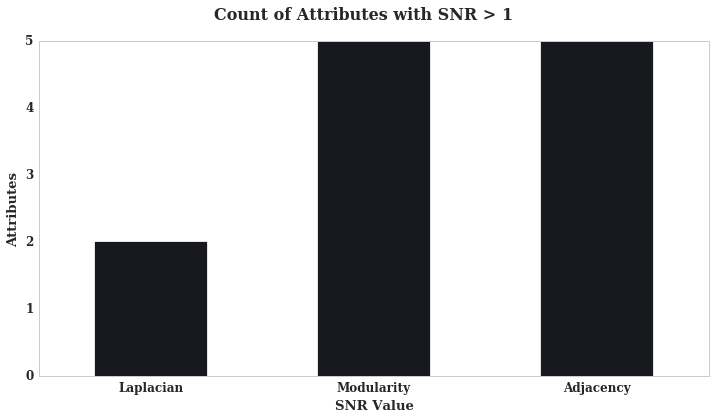
\includegraphics[height =0.3\textheight, width= 0.9\textwidth]{snrcount.png}
    \caption{Plot of Count of Number attributes with $SNR > 1$ from the different graph matrices}
    \label{fig:snr count}
\end{figure}

\begin{figure}[!htp]
    \centering
    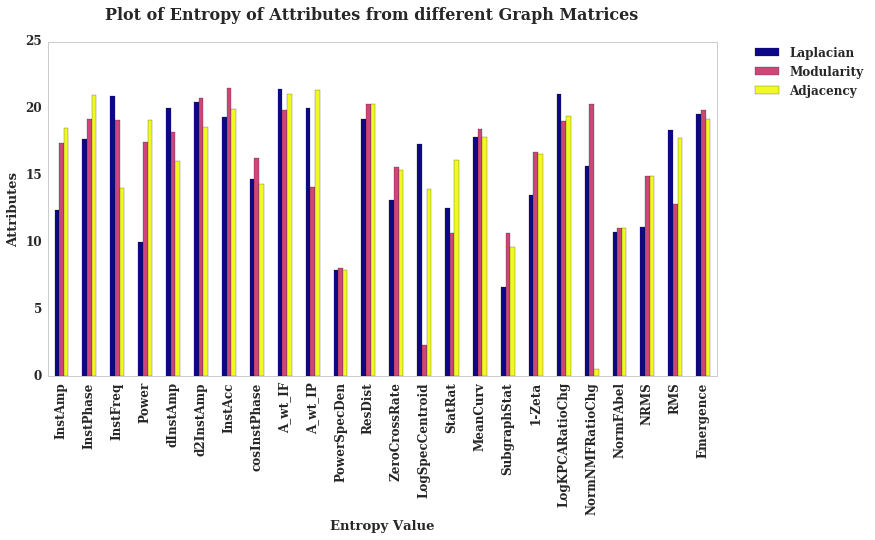
\includegraphics[height =0.5\textheight, width= 0.9\textwidth]{entropy.png}
    \caption{Plot of Entropy of attributes from the different graph matrices}
    \label{fig:entropy}
\end{figure}

\begin{figure}[!htp]
    \centering
    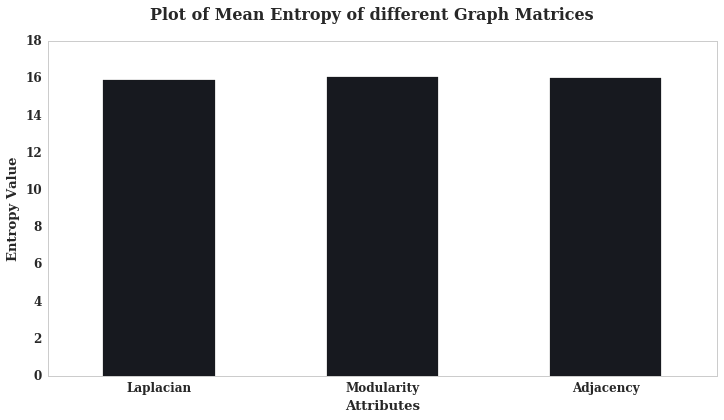
\includegraphics[height =0.4\textheight, width= 0.9\textwidth]{entropy_mean.png}
    \caption{Plot of Mean Entropy of different graph matrices}
    \label{fig:mean entropy}
\end{figure}


\begin{figure}[H]
    \centering
    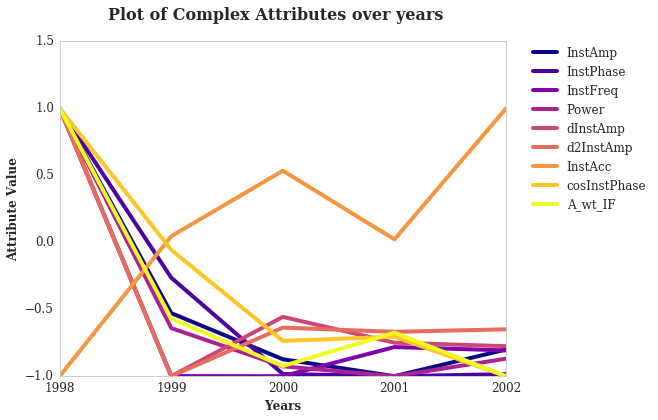
\includegraphics[height =0.4\textheight, width= 0.9\textwidth]{complex_yrs.png}
    \caption{Plot of Complex Attributes over Years}
    \label{fig:complex yrs}
\end{figure}

\begin{figure}[H]
    \centering
    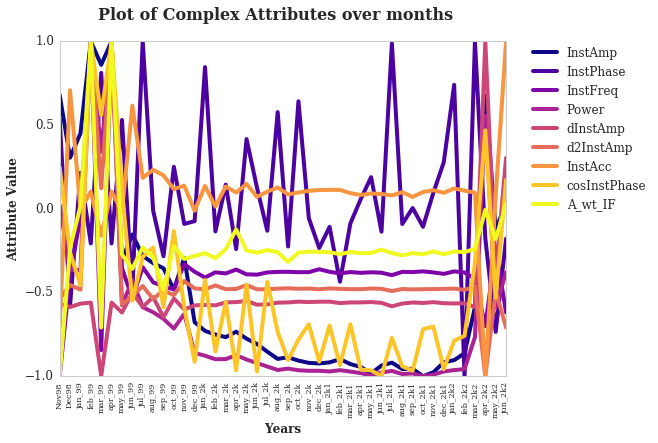
\includegraphics[height =0.4\textheight, width= 0.9\textwidth]{complex_mth.png}
    \caption{Plot of Complex Attributes over Months}
    \label{fig:compolex mth}
\end{figure}


\begin{figure}[H]
    \centering
    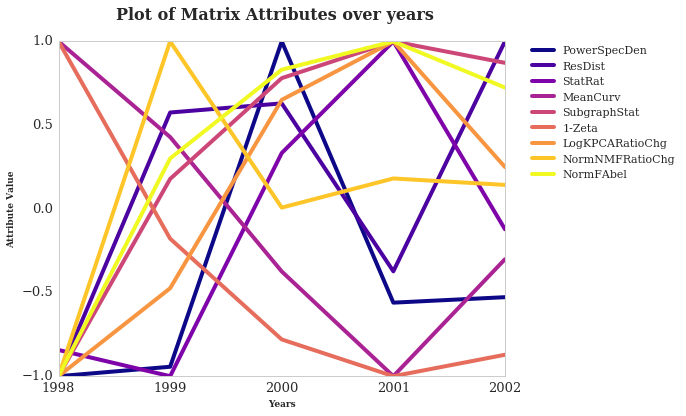
\includegraphics[height =0.4\textheight, width= 0.9\textwidth]{mat_yrs.png}
    \caption{Plot of Matrix Attributes over Months}
    \label{fig:mat yrs}
\end{figure}

\begin{figure}[H]
    \centering
    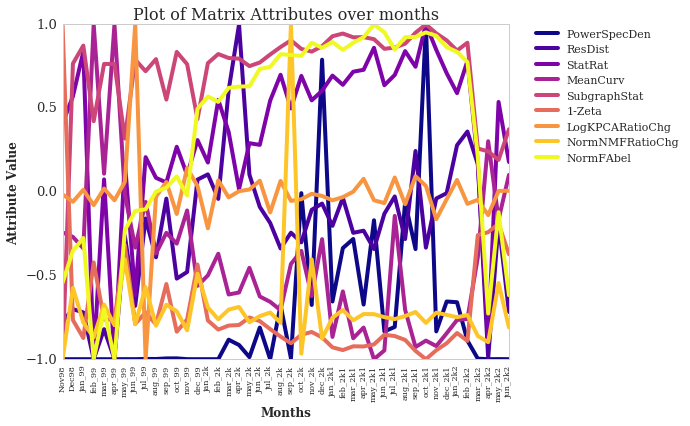
\includegraphics[height =0.4\textheight, width= 0.9\textwidth]{mat_mth.png}
    \caption{Plot of Matrix Attributes over Months}
    \label{fig:mat mth}
\end{figure}

\begin{figure}[H]
    \centering
    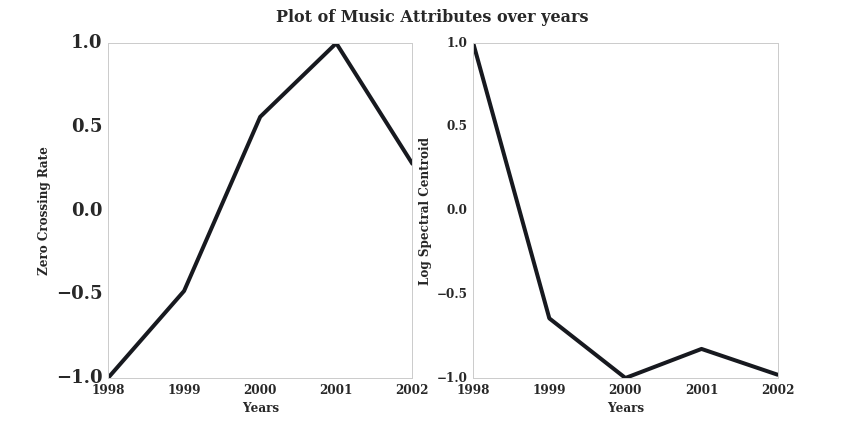
\includegraphics[height =0.4\textheight, width= 0.9\textwidth]{musicatt_yrs.png}
    \caption{Plot of Music Attributes over Years}
    \label{fig:music yrs}
\end{figure}

\begin{figure}[H]
    \centering
    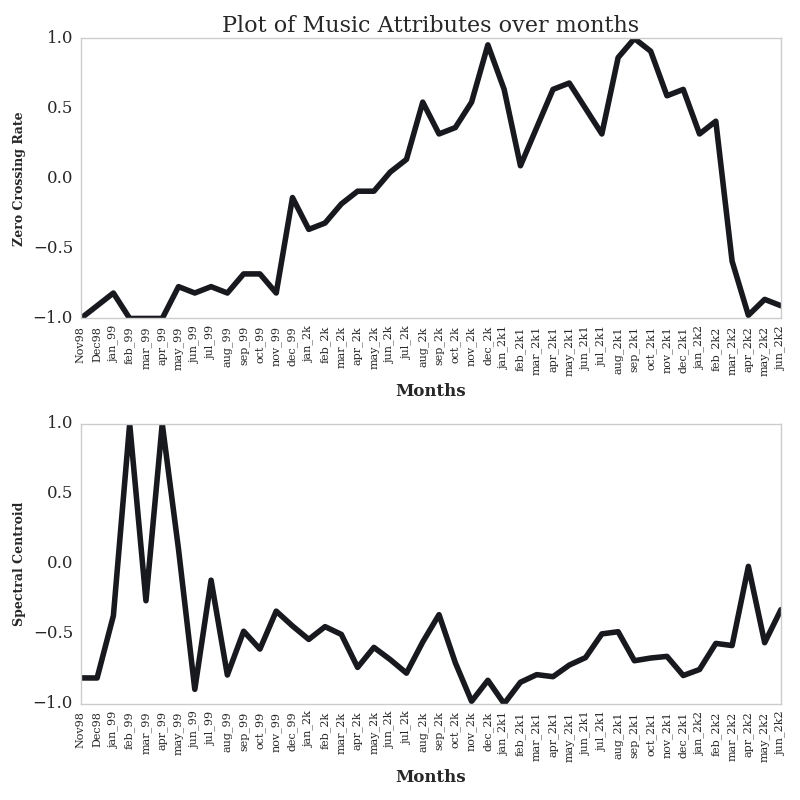
\includegraphics[height =0.4\textheight, width= 0.9\textwidth]{musicatt_mth.png}
    \caption{Plot of Music Attributes over Months}
    \label{fig:music mth}
\end{figure}

\clearpage{}
\subsection{Average Attributes}

\begin{figure}[H]
    \centering
    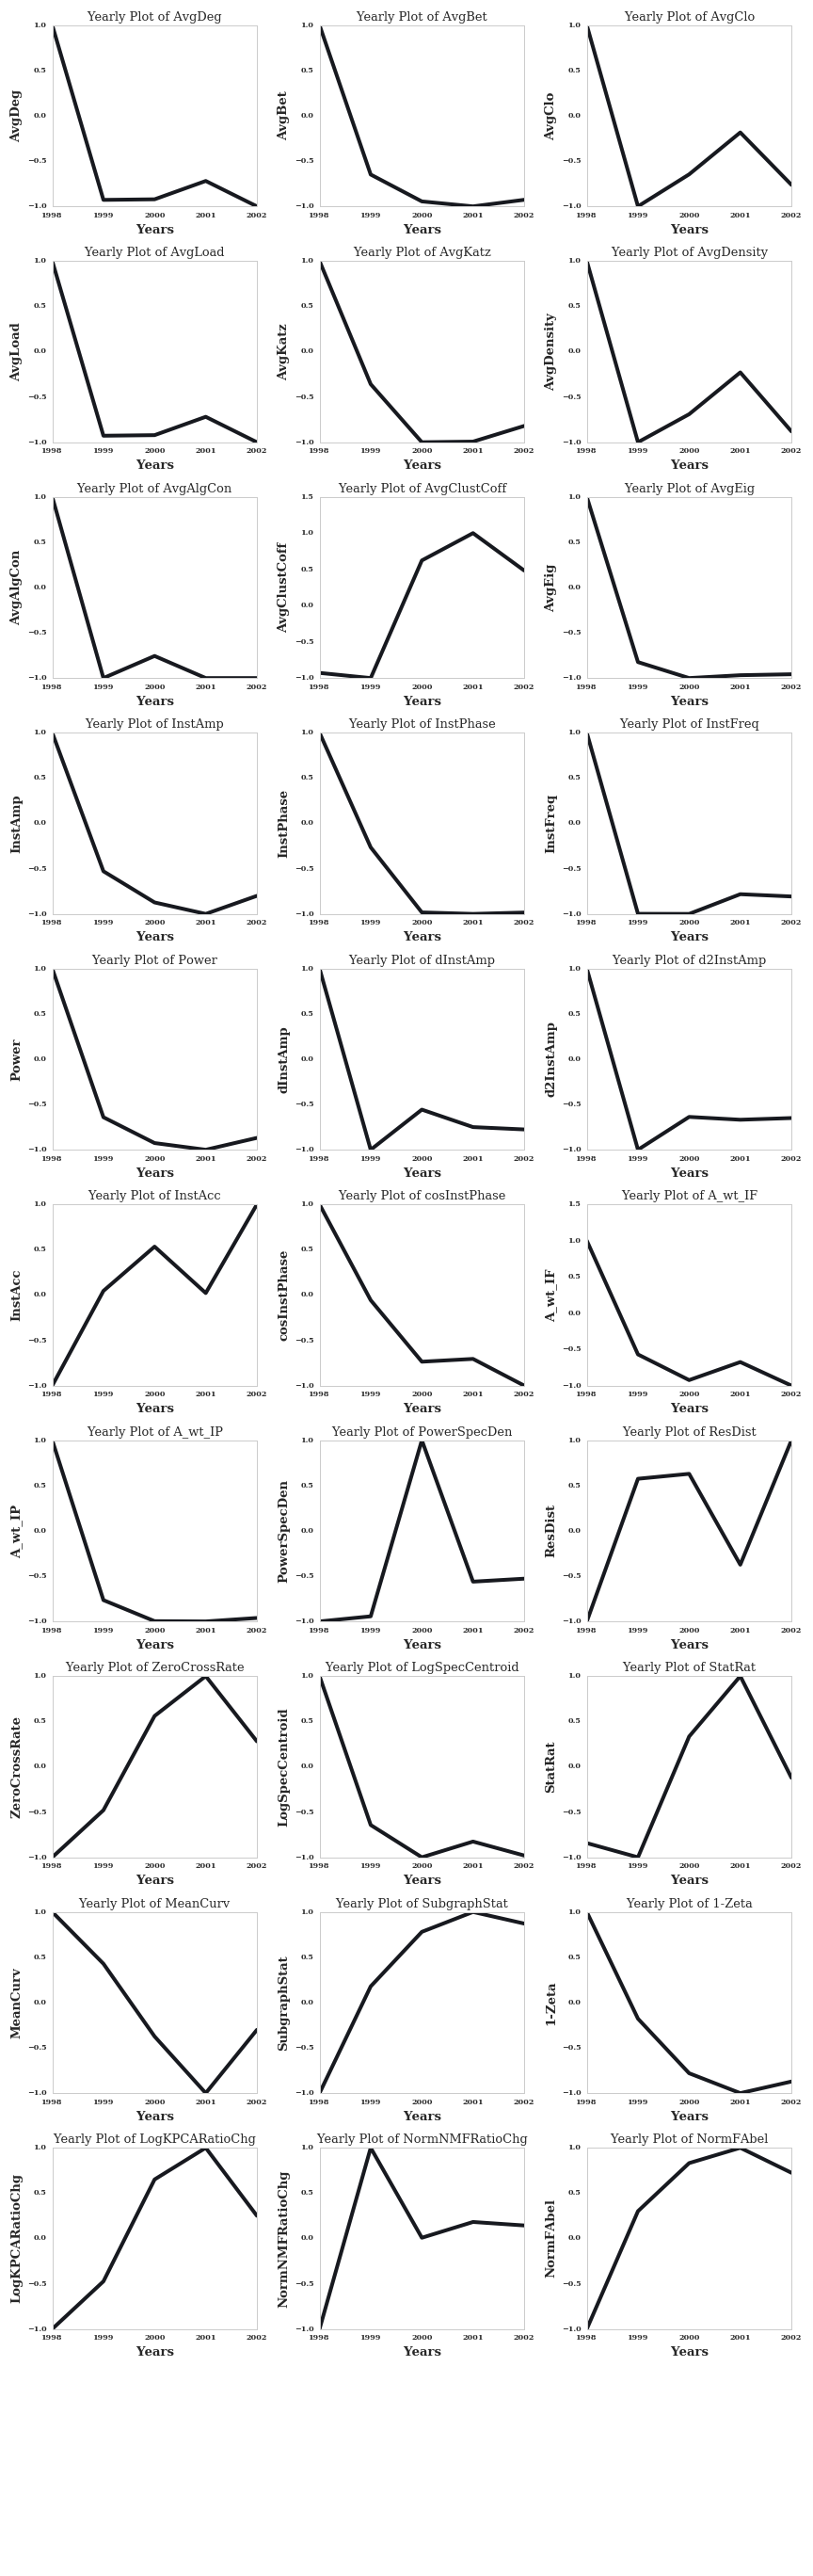
\includegraphics[height =0.9\textheight, width= 0.9\textwidth]{avg_allatt_yrs.png}
    \caption{Plot of Average Attributes over Years}
    \label{fig:avg all yrs}
\end{figure}

\begin{figure}[H]
    \centering
    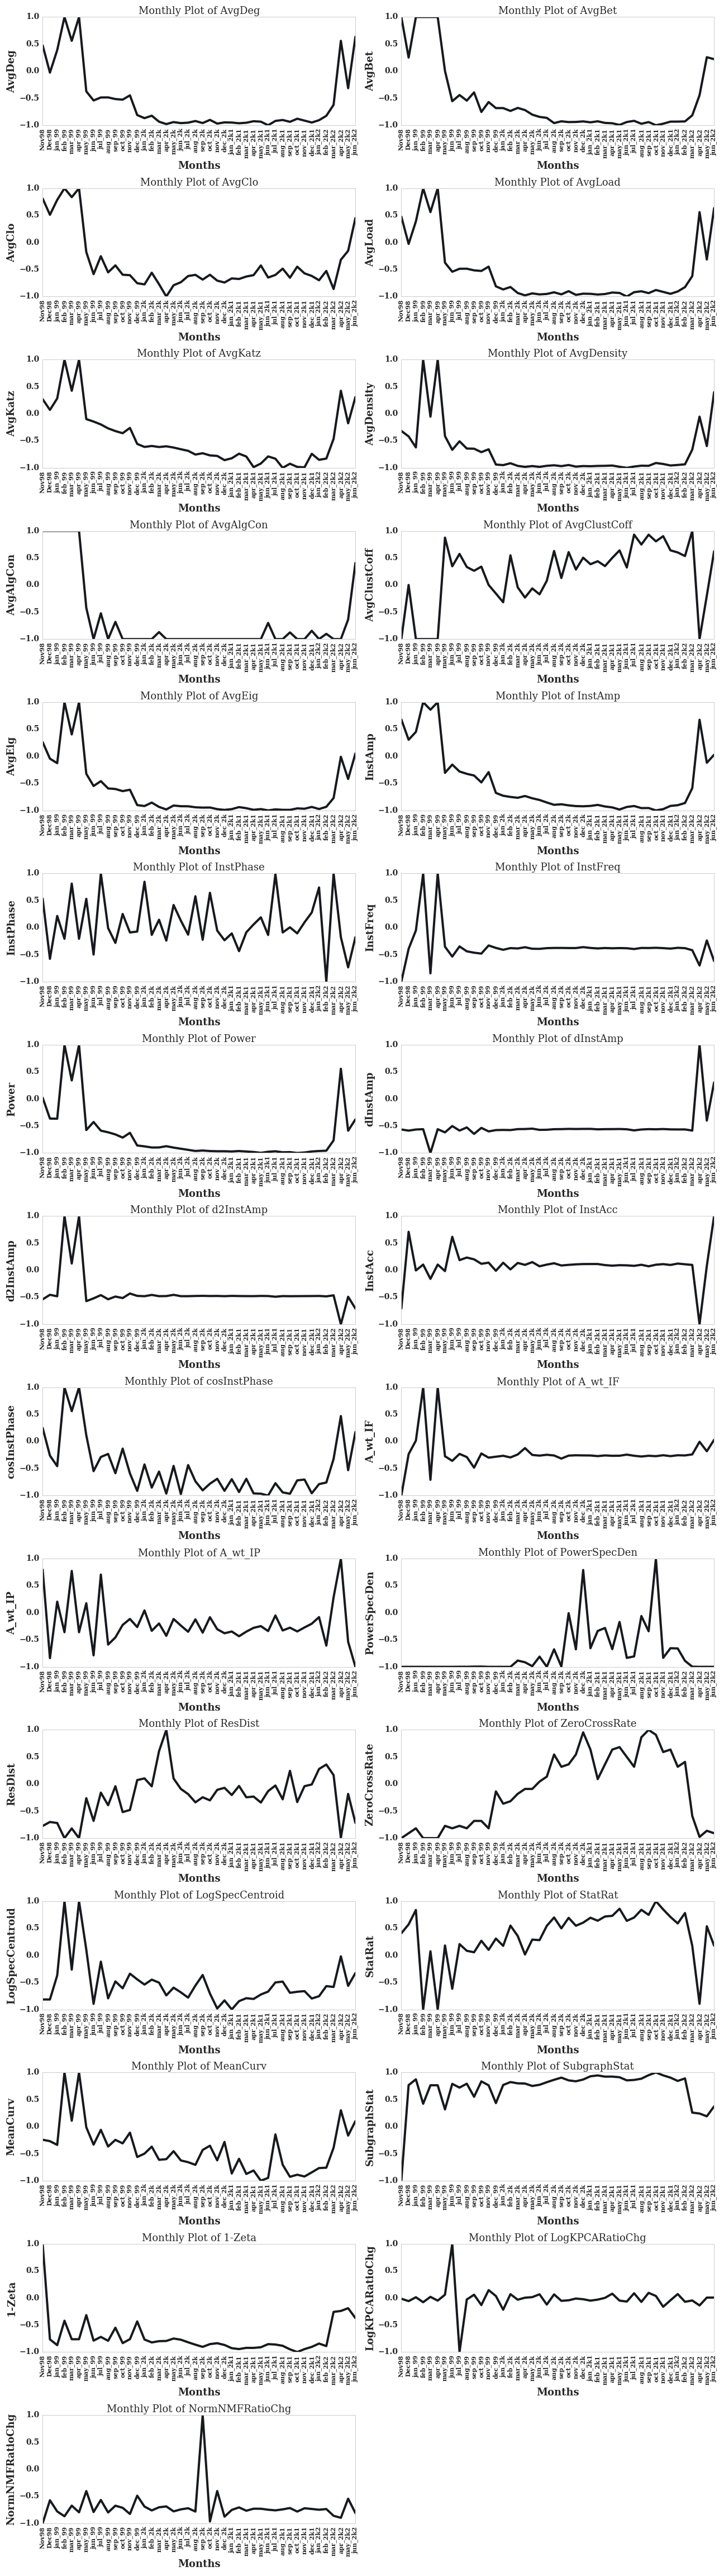
\includegraphics[height =0.9\textheight, width= 0.9\textwidth]{avg_allatt_mth.png}
    \caption{Plot of Average Attributes over Months}
    \label{fig:avg all mth}
\end{figure}

\clearpage{}
\section{Correlation Analysis}\label{corrfig}
 The correlation analysis is performed using the monthly level attributes because the yearly data has a very small sample size. Also the correlation measure used is the Pearson Correlation.\\

\begin{figure}[H]
    \centering
    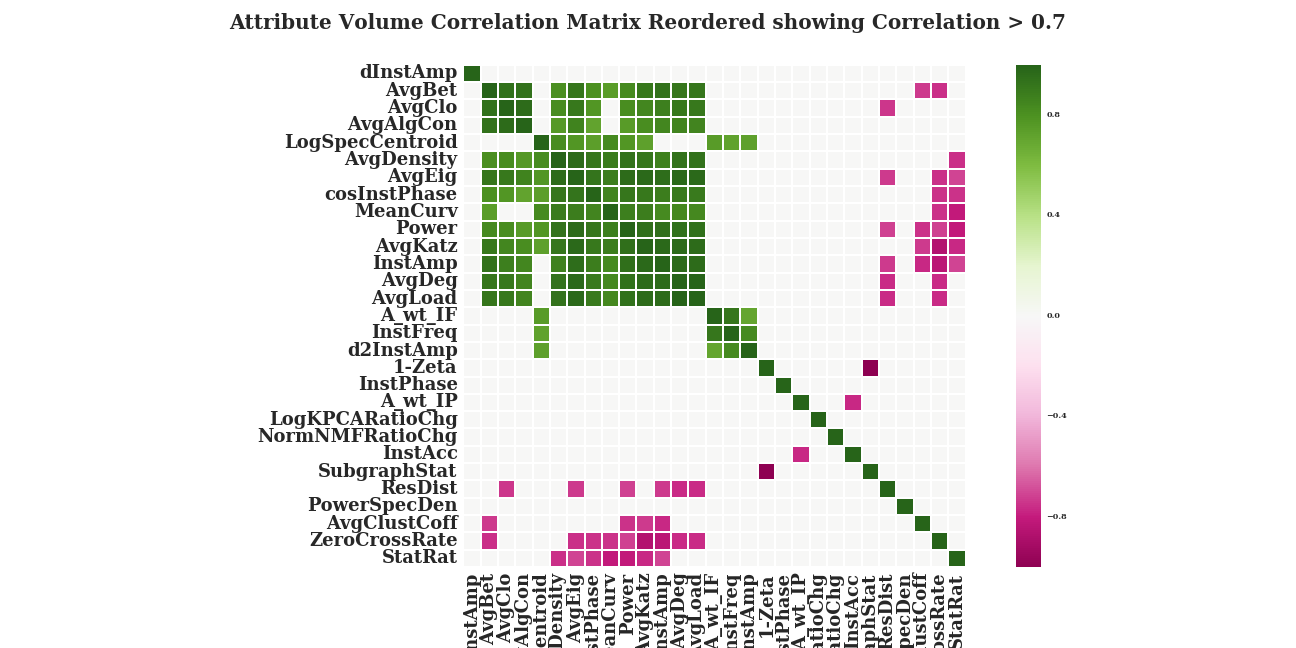
\includegraphics[height =0.8\textheight, width= 1\textwidth]{reordered_corrmat.png}
    \caption{Reordered Correlation Heatmap showing correlation $> 0.7$}
    \label{fig:Corrmat}
\end{figure}

\begin{figure}[H]
    \centering
    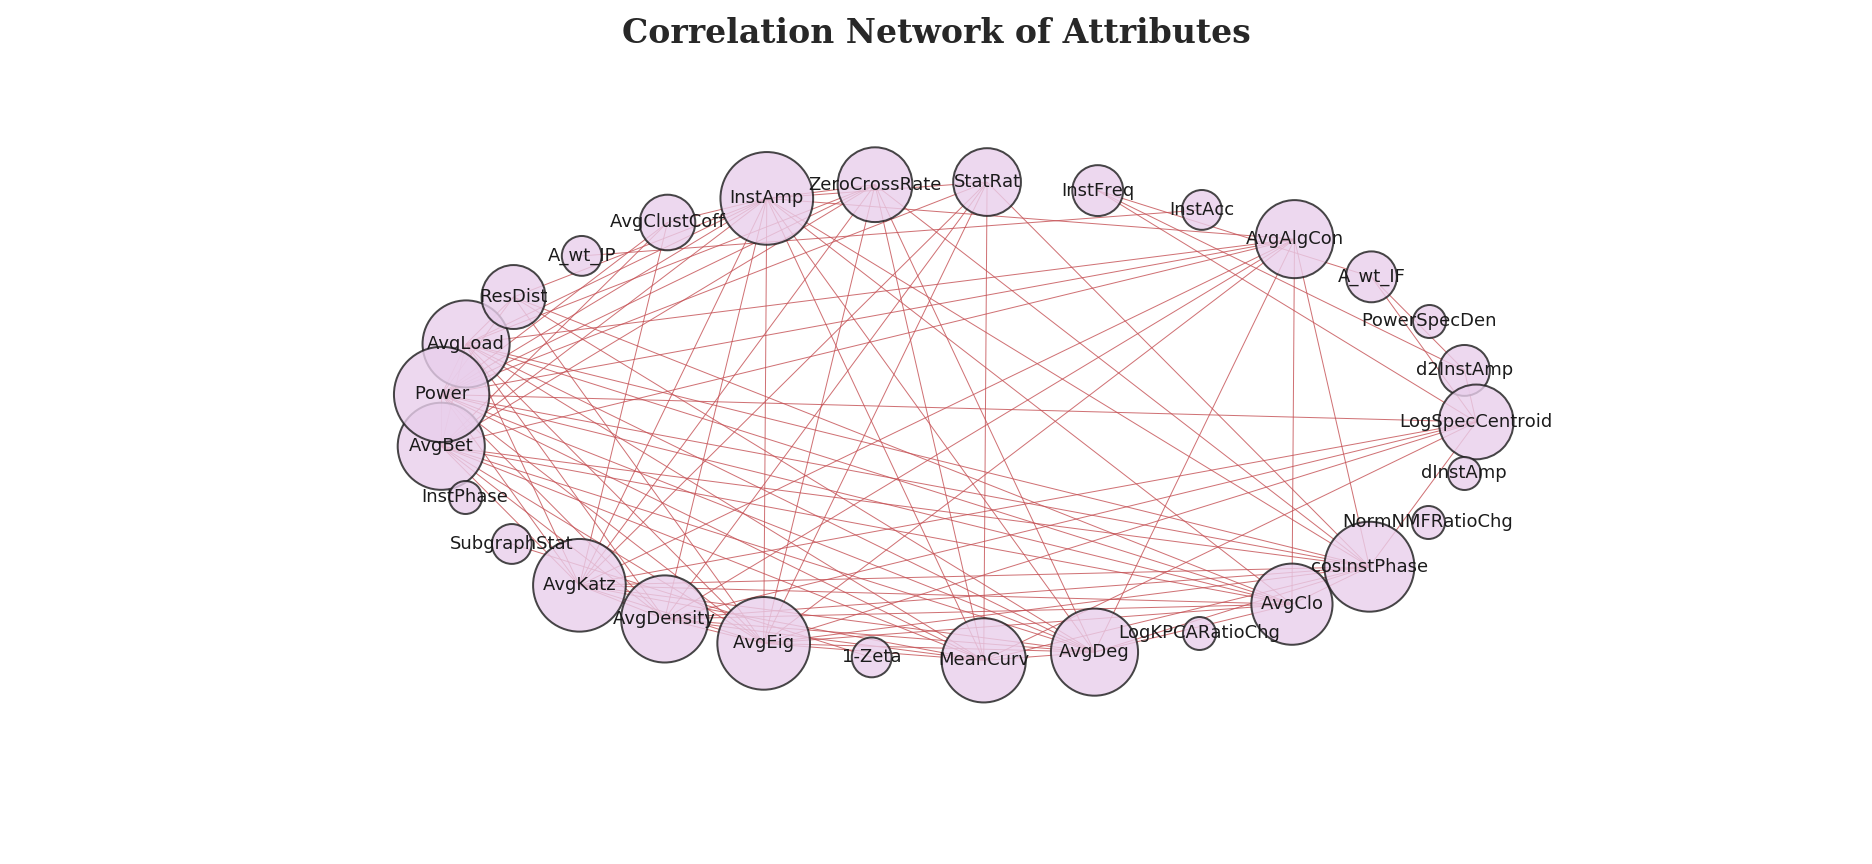
\includegraphics[height =0.4\textheight, width= 1\textwidth]{corrnet.png}
    \caption{Correlation Network of Attributes. The thickness of the borders of the nodes indicates high degree while low thickness of borders around the nodes indicate low degree.}
    \label{fig:CorrNet}
\end{figure}

\begin{figure}[H]
    \centering
    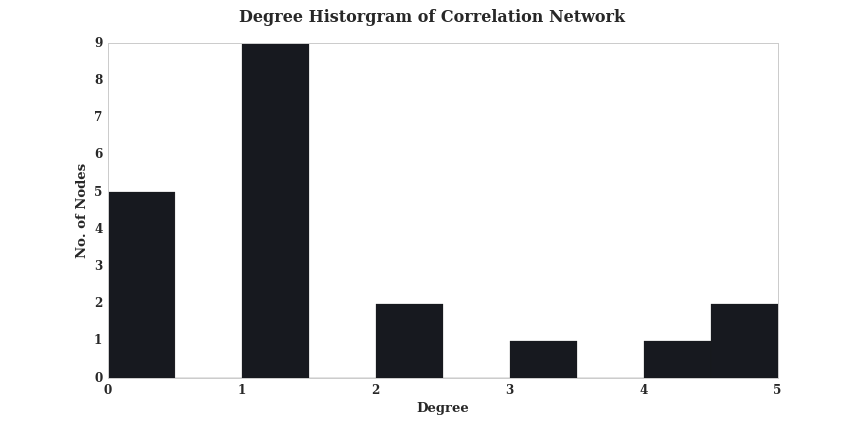
\includegraphics[height =0.4\textheight, width= 0.8\textwidth]{corrnet_deghist.png}
    \caption{Correlation Network Degree Histogram}
    \label{fig:CorrDegHist}
\end{figure}

\clearpage{}
\section{Feature Ranking with Regression Analysis}\label{regplots}

Here I used a Gradient Boosting Regressor with 10 boosting stages to predict the Average Degree of the network using the attribute volume. The test /train split is 50/50 to prevent over fitting. The Regressor produces a feature ranking of the variables and it is very useful to get a sense of the predictive potential of the measures. \\

\begin{figure}[!htp]
    \centering
    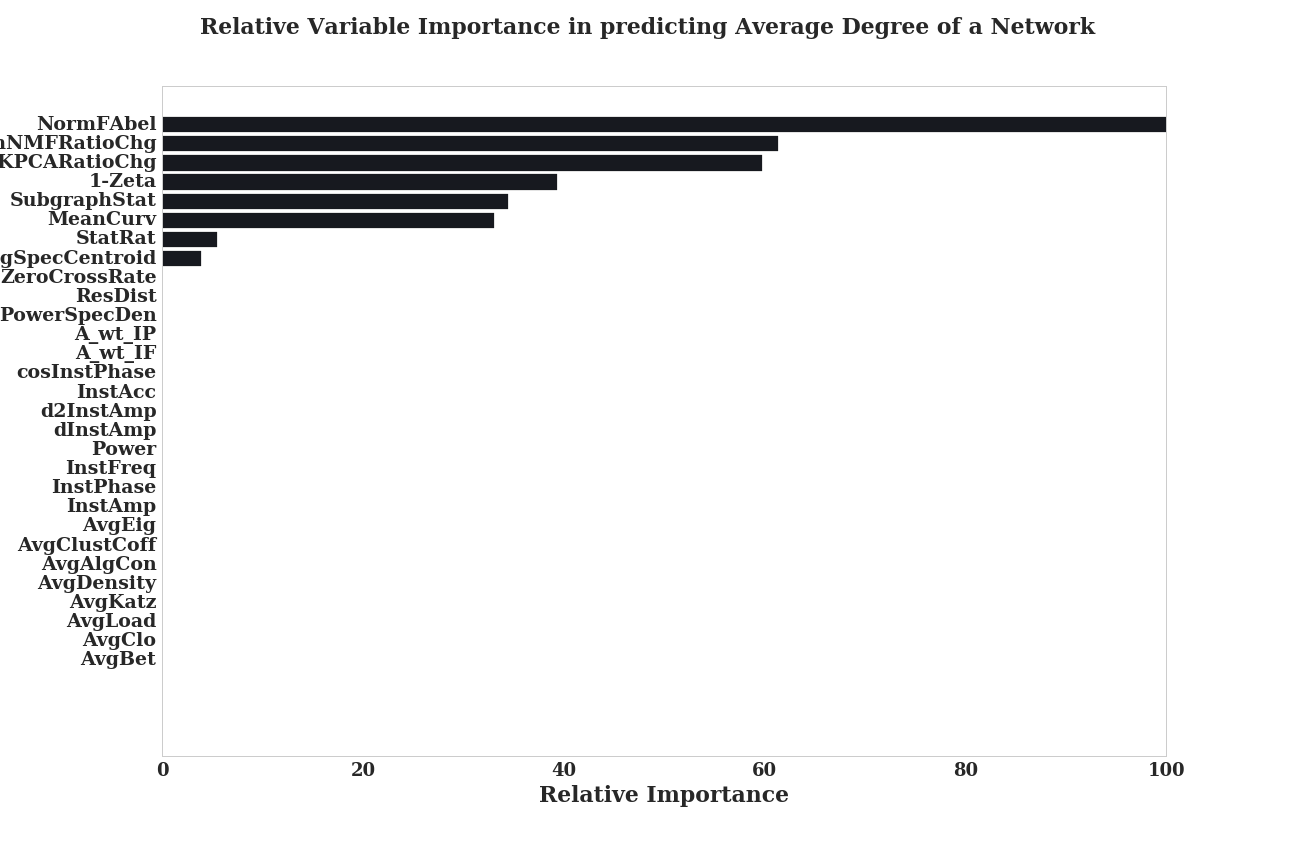
\includegraphics[height =0.5\textheight, width= 0.9\textwidth]{feature_ranking.png}
    \caption{Feature Ranking by Gradient Boosting Regressor for predicting Average Degree}
    \label{fig: featrank}
\end{figure}

\begin{figure}[!htp]
    \centering
    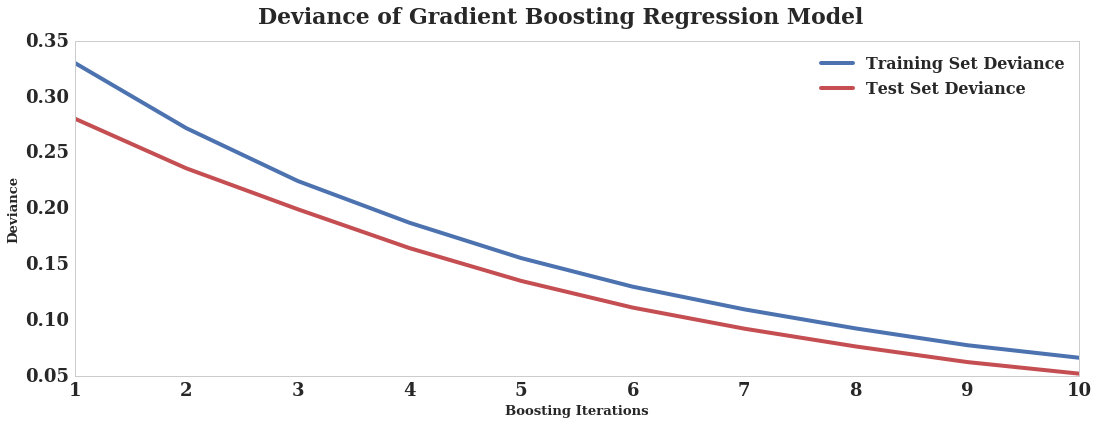
\includegraphics[height =0.2\textheight, width= 0.9\textwidth]{deviance.png}
    \caption{Regression Deviance Plot}
    \label{fig: regdev}
\end{figure}

\clearpage{}
\section{Aggregation Schemes}\label{aggplots}

\begin{figure}[!htp]
    \centering
    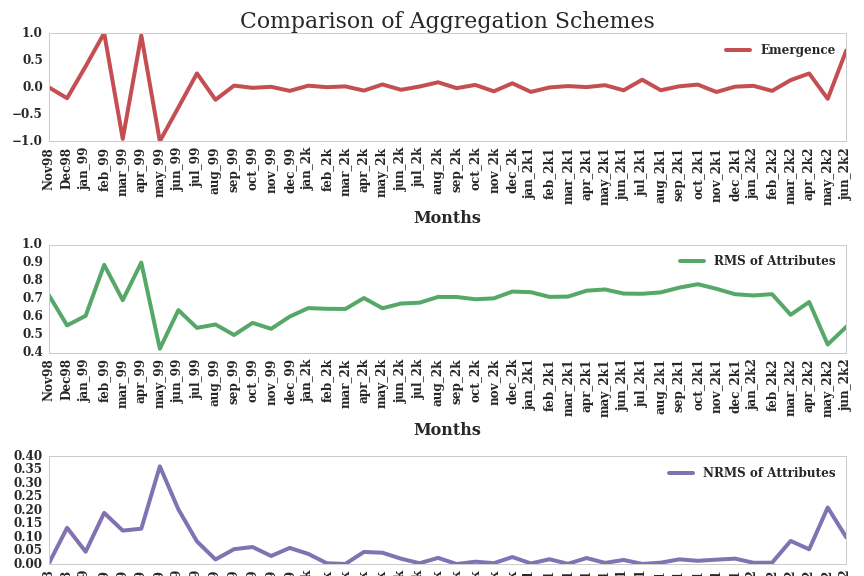
\includegraphics[height =0.9\textheight, width= 0.9\textwidth]{agg_comp.png}
    \caption{Comparison of different aggregation schemes.}
    \label{fig:aggcomp}
\end{figure}

\begin{figure}[!htp]
    \centering
    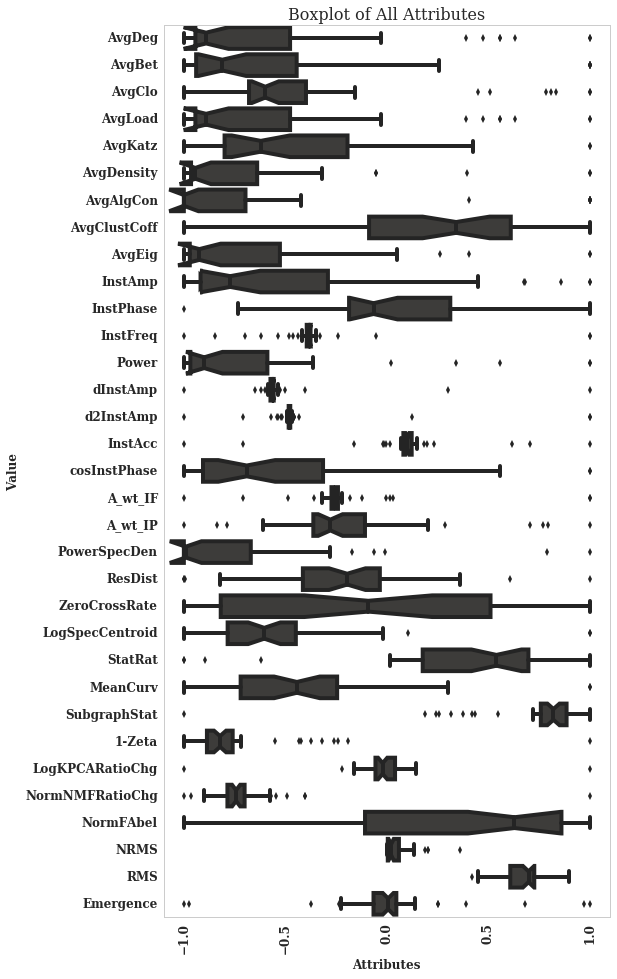
\includegraphics[height =0.9\textheight, width= 0.9\textwidth]{attvol_boxplot_all.png}
    \caption{Boxplot of All Attributes}
    \label{fig:boxplot}
\end{figure}

\clearpage{}
\section{Manifold Visualisation of Attribute Volume}\label{manifoldplots}
\begin{figure}[H]
    \centering
    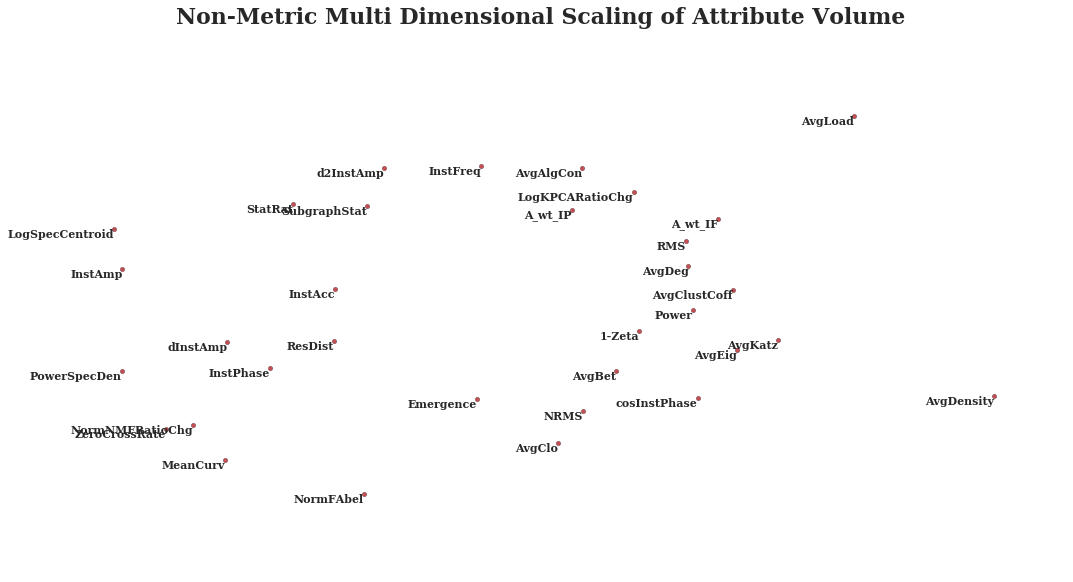
\includegraphics[height =0.4\textheight, width= 0.9\textwidth]{mds.png}
    \caption{Non-Metric Multidimensional Scaling of Attribute Volume}
    \label{fig:MDS}
\end{figure}

\begin{figure}[H]
    \centering
    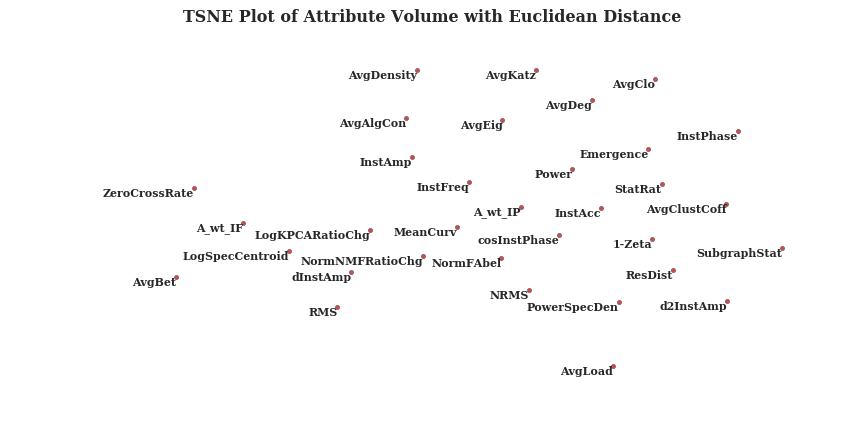
\includegraphics[height =0.4\textheight, width= 0.9\textwidth]{tsne_plot_euc.png}
    \caption{TSNE Plot of Attribute Volume with Euclidean Distance}
    \label{fig:TSNE Euclid}
\end{figure}

\begin{figure}[H]
    \centering
    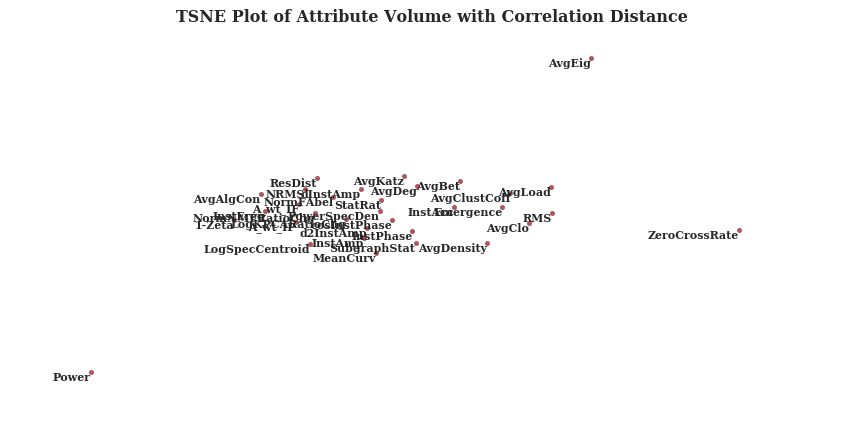
\includegraphics[height =0.4\textheight, width= 0.9\textwidth]{tsne_plot_corr.png}
    \caption{TSNE Plot of Attribute Volume with Correlation Distance}
    \label{fig:TSNE}
\end{figure}

\begin{figure}[H]
    \centering
    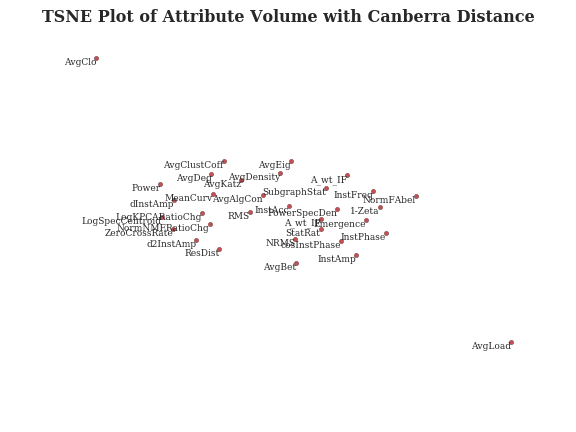
\includegraphics[height =0.4\textheight, width= 0.9\textwidth]{tsne_plot.png}
    \caption{TSNE Plot of Attribute Volume with Canberra Distance}
    \label{fig:TSNE}
\end{figure}

\clearpage{}
\section{FK and Radon Plots}\label{seisplots}

\begin{figure}[!htp]
    \centering
    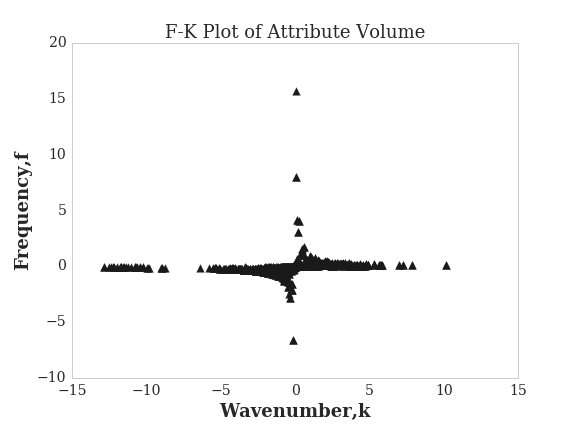
\includegraphics[height =0.4\textheight, width= 0.9\textwidth]{fkplot.png}
    \caption{Frequency Wavenumber (FK) Plot of Attribute Volume}
    \label{fig: fkplot}
\end{figure}

\begin{figure}[!htp]
    \centering
    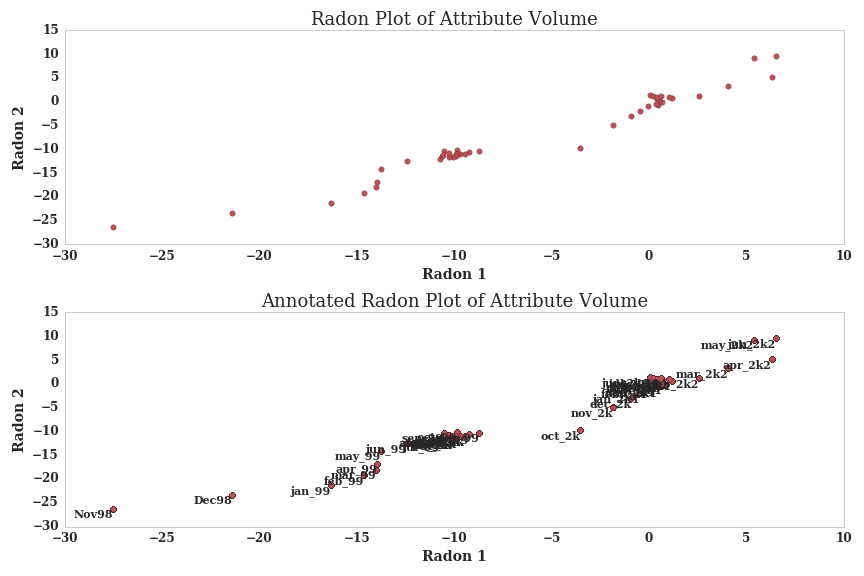
\includegraphics[height =0.4\textheight, width= 0.9\textwidth]{radonplot.png}
    \caption{(top) Radon Plot of Attribute Volume, (bottom) Annotated Radon Plot}
    \label{fig: radonplot}
\end{figure}


\begin{figure}[!htp]
    \centering
    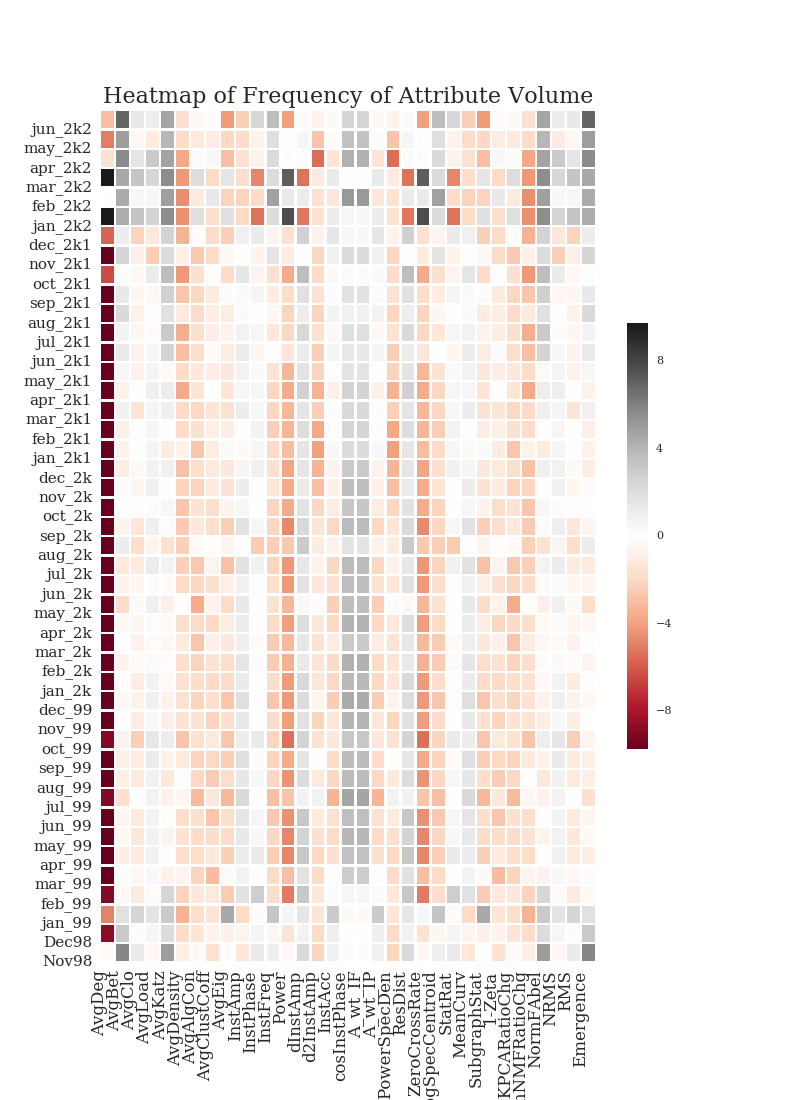
\includegraphics[height =0.4\textheight, width= 0.9\textwidth]{freq_heat.png}
    \caption{Heatmap of Frequency of Attribute Volume. This is the F component derived from the FK Plot}
    \label{fig:Frequency Heatmap}
\end{figure}

\begin{figure}[!htp]
    \centering
    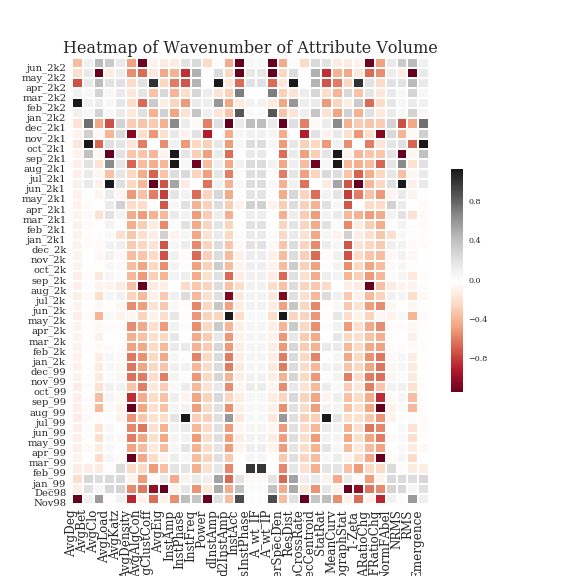
\includegraphics[height =0.4\textheight, width= 0.9\textwidth]{wavnum_heat.png}
    \caption{Heatmap of Wavenumber of Attribute Volume. This is the K component derived from the FK Plot}
    \label{fig:Wavenumber Heatmap}
\end{figure}

\begin{figure}[!htp]
    \centering
    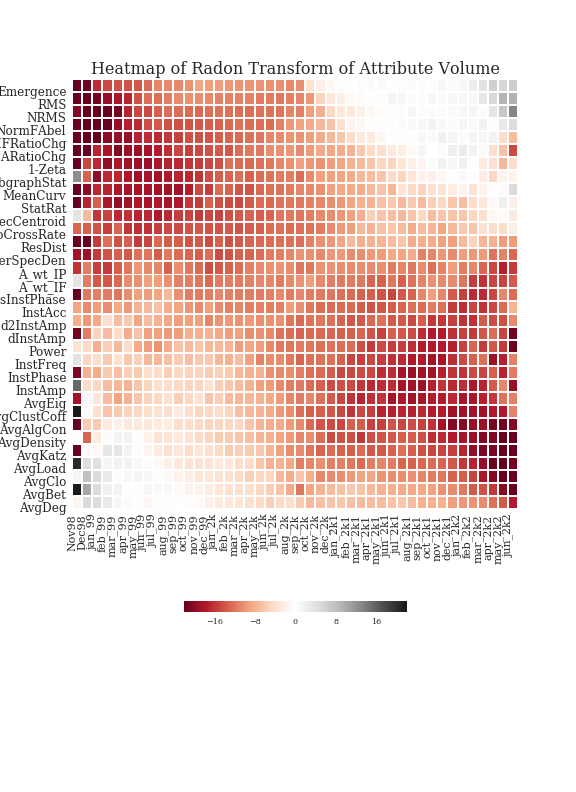
\includegraphics[height =0.7\textheight, width= 0.9\textwidth]{radon_heat.png}
    \caption{Heatmap of Radon Transform of Attribute Volume}
    \label{fig: Radon Heatmap}
\end{figure}

\begin{sidewaysfigure}
    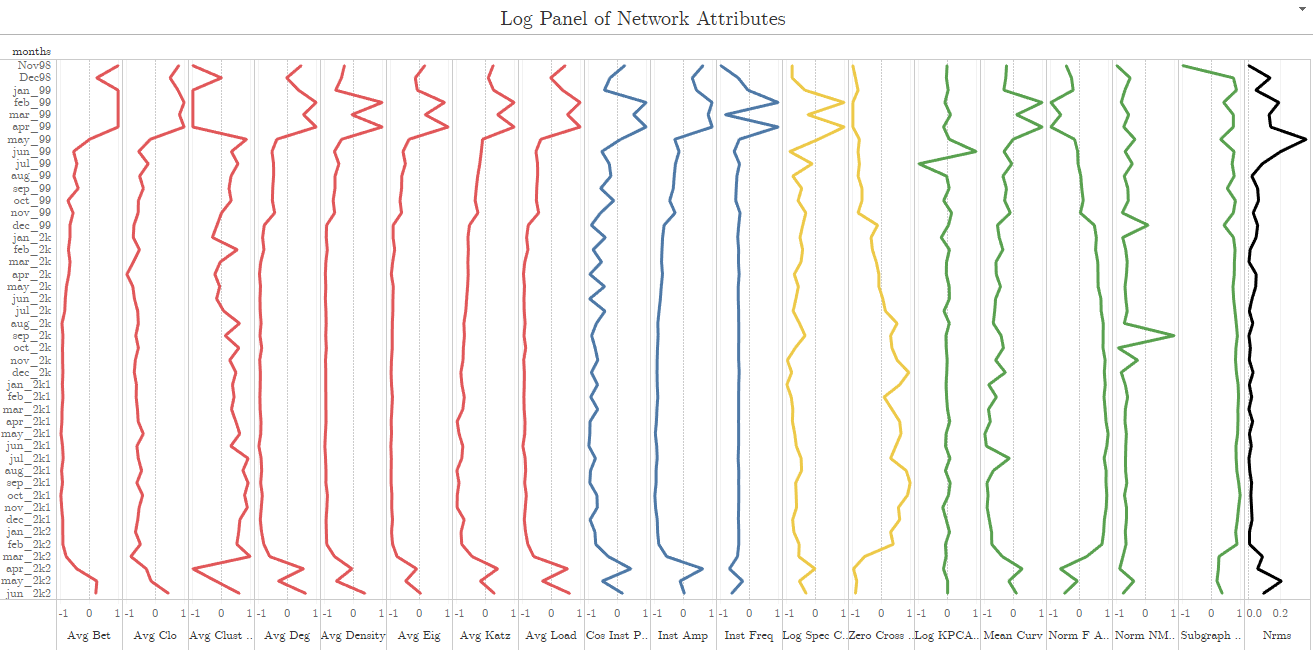
\includegraphics[width=\textwidth]{logpanel.PNG}
    \caption{Log Panel of selected attributes. Benchmark attributes are shown in red. Seismic Attributes shown in blue. Music Attributes shown in yellow. Matrix Attributes shown in green and NRMS aggregation measure in black.}
    \label{fig: logpanel}
\end{sidewaysfigure}

\clearpage{}
\section{Node Level Trends}\label{nodeplots}

In this section I find common nodes across the 5 years and compare their centrality trends over time. The yearly trends for this part of the analysis is conducted as this is more plausible. The reason being that although these nodes are common across the years they do not have activity regularly across all months. Therefore it is deemed more informative to get an overview of their yearly centrality measure changes.\\

\begin{figure}[!htp]
    \centering
    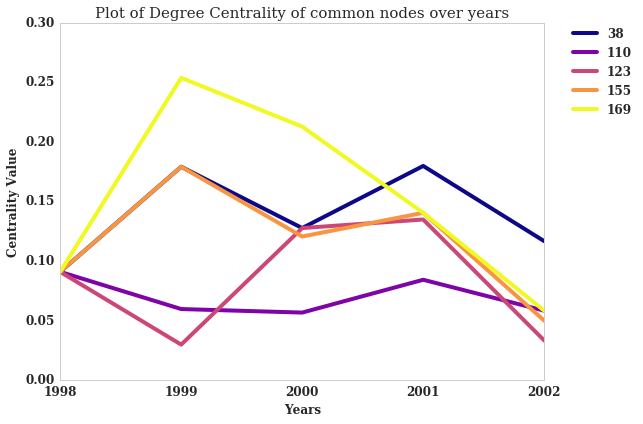
\includegraphics[height =0.3\textheight, width= 0.7\textwidth]{node_deg.png}
    \caption{Plot of Common Node Degree over years}
    \label{fig: Plot of Common Node Degree Centrality over years}
\end{figure}

\begin{figure}[!htp]
    \centering
    \includegraphics[height =0.3\textheight, width= 0.7\textwidth]{node_bet.png}
    \caption{Plot of Common Node Betweenness Centrality over years}
    \label{fig: Plot of Common Node Betweenness Centrality over years}
\end{figure}

\begin{figure}[!htp]
    \centering
    \includegraphics[height =0.4\textheight, width= 0.7\textwidth]{node_clo.png}
    \caption{Plot of Common Node Closeness Centrality over years}
    \label{fig: Plot of Common Node Closeness Centrality over years}
\end{figure}

\begin{figure}[!htp]
    \centering
    \includegraphics[height =0.4\textheight, width= 0.7\textwidth]{node_eig.png}
    \caption{Plot of Common Node Eigenvector Centrality over years}
    \label{fig: Plot of Common Node Eigenvector Centrality over years}
\end{figure}

\begin{figure}[!htp]
    \centering
    \includegraphics[height =0.4\textheight, width= 0.7\textwidth]{node_katz.png}
    \caption{Plot of Common Node Katz Centrality over years}
    \label{fig: Plot of Common Node Katz Centrality over years}
\end{figure}

\begin{figure}[!htp]
    \centering
    \includegraphics[height =0.4\textheight, width= 0.7\textwidth]{node_load.png}
    \caption{Plot of Common Node Load Centrality over years}
    \label{fig: Plot of Common Node Load Centrality over years}
\end{figure}

\clearpage{}
\section{Discussion of Results}

In this section we have shown the results of the methods discussed extensively in Chapter 3. To begin with we started with some familiar visualisations such as node link and matrix diagrams of the networks at the yearly and monthly intervals. These are denoted in \Cref{fig:Node Link Diagram for the yearly networks,fig:node mth,fig:Reordered Matrix Diagram for the yearly networks,fig:Reordered Matrix Diagram for the monthly networks}.\\

From the yearly plots we see that the network is most sparse in 1998 and gradually gets more dense throughout the time period and then shrinks again in 2002. This is reflected in the waveform plots in  \Cref{fig:Audio Waveform Plot for the yearly networks,fig:Audio Waveform Plot for the monthly networks}. Here we see that the signal for 1999 is very blocky indicating probably that not many nodes are present in the network hence the amplitude envelope is smooth and blocky. But in the cases where the networks are dense we see that the signal is spiky indicating the greater number of nodes who have an associated amplitude and some have higher amplitude than others. These nodes are probably the more central players in the network. This is reflected at the monthly level as well as the first few months of the graph time series the networks are comparatively sparse compared to the middle. The network starts to thin out in the last few months of the time range. \\

The exploratory centrality histograms at the year and monthly level are what is observed in networks more generally. This is that they exhibit a long tail with most nodes having low values and some nodes having high values. The only other key observation from the figures in \Cref{explanal} are the extremes at the beginning of the time series where the networks are thin. This is reflected by the small number of nodes overall in both the monthly and yearly networks. In the case of the monthly networks a similar trend is observed where there are an overall smaller number of nodes due to thinning of the network which results in a sort of bimodal appearance of the centrality histograms. For most of the time series we see the long tail in centrality value distribution. \\

A key component of the analysis of the novel measures proposed in this study was to compare their behaviour to a set of benchmark measures. These measures are shown for the yearly and monthly networks in \Cref{bmark}. From the yearly level plot \Cref{fig:bmark yrs} we see that the change point in the network is the year 1999 and 2001. The network seems to be expanding from 1999 by all measures and contracting from 2001 onwards. From the monthly plot \Cref{fig:bmark mth} we see an interesting structure emerge. The graph time series seems to be characterised by two large peaks for the Feb - Apr 1999 period and two slightly smaller peaks between Apr 2002 and June 2002. In addition Feb 2000 appears to be interesting but only the Average Clustering Coefficient highlights this period with any conviction out of the benchmark metrics. Therefore, we expect our new measures at a minimum to replicate these features and highlight any additional ones. \\

In the figures in \Cref{attanal} we highlight the steps undertaken to decide which graph matrix to use for the derivation of the attributes. From the three matrices: Normalised Laplacian, Modularity and Adjacency we chose the Normalised Laplacian. The reasoning for this is highlighted in \Cref{fig:snr,fig:snr count,fig:entropy,fig:mean entropy}. The first step was to look at the Signal to Noise ratio of all the proposed attributes calculated from the different matrices. The reasoning being that high SNR means better attributes. By this account it would appear that the Modularity and Adjacency matrices would be better choices because they have higher number of attributes with high SNR compared to the Laplacian. However, upon closer inspection of both the high and low SNR attributes we found this to be a bit misleading. The attributes which have low SNR from the Modularity and Adjacency matrices fail to recover the signal we established. But the attributes with high SNR to do this well. However for the Laplacian attributes the low SNR attributes are able to recover the signal that the same attributes from the other matrices are not. This can be seen in detail from Appendix E. So we decided to refine our analysis and consider another information theoretic measure, Entropy. From the Entropy plots we see that all three matrices seem to be similar with respect to their average Entropy but the Laplacian has lower average Entropy meaning lower uncertainty compared to the other two matrices. This combined with the observation that the attributes from the Laplacian are better at recovering the signal observed in the benchmark measures. We us the Laplacian attributes in all further results that are presented. \\

The Complex attributes are the first of the Seismic Attribute that we present. From \Cref{fig:complex yrs,fig:compolex mth} we see that the prominent peaks are retrieved by all the measures clearly with the Amplitude and the Cosine of Instantaneous Phase highlighting additional areas hinted at by the Average Clustering Coefficient. For the yearly the the 1999 change point is very clear among all the measures and suggests the network is contracting from 2001 onwards. Both sets of measures agree that the most significant time period is 2001.  \\

The matrix attributes shown in \Cref{fig:mat yrs,fig:mat mth} are also interesting in the sense that they also retrieve the key structures but are more smooth in general compared to the complex trace attributes. For the matrix attributes at the year level we see a large number of them converge to a peak in 2001 while a few converge to a trough. This is indicating the same phenomenon although with the opposite polarity. The monthly plot highlights the strong peaks as with the other attributes but in addition Nov 2000 and Oct 2001 are indicated to periods of strong change. Although the Average Clustering Coefficient indicates these periods it does not mark these periods as strongly as the matrix attributes but finds them to be roughly similar. So here we have a means of gaining additional insight into some of the structure suggested by the benchmark measures. These periods also do not show particularly strongly among the centrality measures.\\

The music attributes shown in \Cref{fig:music yrs,fig:music mth} are also able to retrieve the structure observed in the benchmark measures convincingly. From both the Zero Crossing Rate and the Spectral Centroid attribute we see they agree on the yearly peak being the year 2001 and declining thereafter. Interestingly the Zero Crossing Rate finds the peaks in the early and later part of the monthly time series but the peaks are smaller indicating that since the networks are smaller at these steps there are a a limited number of crossings available compared to when the network is larger and the signal is longer. Hence this makes sense in the context of the peaks later in the time series where the networks are denser. The Spectral Centroid shows a familiar structure while finding the additional peaks we have identified from the benchmark, complex and matrix attributes. \\

Of the remaining attributes shown in \Cref{fig:avg all yrs,fig:avg all mth} we some interesting behaviour for example the KLPCA Ratio is used to detect unconformities. Unconformities are breaks in the depositional surface separating the rock masses into two different ages. This indicates a break in the sedimentation sequence. In our case we can think of the unconformity as being a large break. Therefore it is interesting to see that the change points in 1999 are highlighted very well by this attribute.  \\

The Phase attributes such as Instantaneous Phase, Cosine of Instantaneous Phase and Amplitude Weighted Instantaneous Phase have similar behaviour in the sense that they are sensitive to other changes apart from the instances when the network is small such as in early 1998. We see that the Phase attribute suppresses the two peaks when the network is really small but highlights other changes along the time series. However, this attribute is rather noisy so typically in a seismic attribute analysis the Cosine of Phase is used as it is better constrained and the polarity can be controlled. In this study we choose to look at peaks but one could easily flip the sign and look at troughs. This attribute is less noisy and is sensitive to the big and small changes in the network. The Amplitude weighted Phase attribute also highlights the bigger changes while suppressing the smaller changes. This is hardly surprising as the Amplitude attribute finds the amplitude anomalies in the network which are at the beginning and end of the series. The first and second derivatives of the Amplitude are smoother versions of the Amplitude and find the greatest change in the Amplitude while suppressing smaller changes. \\

The Frequency and Frequency derived attributes is smooth attribute that also highlights the biggest change periods in the network. The derivative of the Frequency Instantaneous Acceleration however is more interesting as it is able to provide additional granularity to the periods that the Frequency attribute highlights as having the greatest change. For example in the period from 1998 to early 1999 we see the two peaks in the Frequency but the Acceleration highlights within this time frame that Dec 98 and May 99 are particularly significant. The May 99 period is hinted at by the Frequency but its magnitude compared to the neighbouring periods is lower. The Amplitude weighted Frequency shows a similar propensity of being more sensitive to big change points.\\

The Stationarity measures such as the Subgraph Stationarity, Stationarity Ratio, 1-Zeta show the change points along the time series but capture slightly different dynamics. The 1- Zeta which gives a sense of how the members have changed between time periods rightly highlights the periods of expansion early and contraction later in the series. Where the network is fairly dense the attribute is smooth. The Subgraph stationarity which utilises the union and the intersection of adjacent graph matrices also captures this dynamics that the graph dissimilarity shows as a trough, while similarity shows as a fairly flat line. The Stationarity is more sensitive in the sense that the contractions in the network show as large troughs while the expansion shows a largely positive trend. \\

The Power attributes such as the Power and Power Spectral Density are interesting that while the Power attributes behaves largely like a smoother Amplitude attribute with the large changes enhanced. The Power Spectral Density is less sensitive to these contraction changes but rather highlights structure in the dense parts of the network which the other attributes do not do as well. The Power Spectral Density and the Zero Crossing Rate are similar in this respect. Both these attributes find greater changes in denser part of the network. \\

The Norm of the Forward Abel Transform of the magnitude of the Fourier Transform (Norm FAbel) captures the trend established from all the metrics so far the best. This is because the early part of the network, when it is small show up as troughs which are smaller in magnitude that those at the denser part of the network when it is expanding and also much smaller than the period in the end when the network is contracting again. \\

The Resistance Distance and Curvature measures also highlight the periods of greatest change and more sensitive to large changes in both the dense and sparse parts of the network. For example the Mean Curvature best highlights the Aug -  Sep 2001 change period most clearly out of all the attributes. The Resistance Distance likewise highlights the Mar - Apr 2000 period as being significant more clearly than most other attributes.\\

The figures in \Cref{corrfig} shows the Pearson Correlation among the different attributes. The correlation matrix shown in \Cref{fig:Corrmat} shows the correlations above 0.7 and everything else has been set to zero. This allows us to see to the highly correlated items only. Also a hierarchical clustering is used to groupd the variables and then these indices are used to sort the rows and columns of this matrix so we are able to derive a reordered correlation matrix showing the high and low correlation items in clear clusters. As an extension to this analysis we take this matrix and derive a correlation network of attributes. Here the degree of a node is determined by the number of other nodes that it is highly correlated with. So in \Cref{fig:CorrNet} we see the network with the Degree encoded as the thickness of the border of the nodes. From \Cref{fig:CorrDegHist} we see that 9 attributes have at least 1 other attribute that they are correlated with 5 attributes being completely disconnected such as the Power Spectral Density, Log KLPCA Ratio Change, NMF Ratio Change and Derivative of Instantaneous Amplitude. A small number of attributes have very high Degree such as Power. We could say that a lot of the metrics capture similar information to the centrality measures even though the way they are calculated are very different. \\

The Regression method used for the results in \Cref{regplots} are from a Gradient Boosting Regressor which is mainly used for feature ranking. The dataset size is limited since we are only working with 44 monthly networks with a total of 30 attributes. To get a good idea of feature importance and prevent over fitting we separate the data into 50/50 test/train chunks. The aim was to rank features by importance in predicting a fundamental property such as Average Degree. We see predict these fundamental properties for a graph time series with reasonable accuracy ($> 95pc$). From the feature ranking we see that the features that are not well correlated to other features are paticularly important in this predictive model. Also we noted earlier that the Abel Transform attribute captured the insight we gained from the network visualisations that the early part of the network was sparse compared to the later parts so it is encouraging to see that this attribute is capturing useful dynamics from a predictive context as well. \\

In \Cref{aggplots} we show the aggregation measures proposed in this study the RMS and NRMS in addition to the Emergence measure proposed in literature. The Emergence measures as expected shows the bursts really clearly but the rest of the changes are fairly damped. The RMS is better in this respect that the bursts as well as the drop due to the sparsification towards the end of the time range. The period of densification is also clear from the positive trend. The NRMS is constrained in this case between [0, 0.4] so it is easier to interpret changes from zero. The NRMS measure segments the time series into periods of large and smaller changes. When the networks are or similar size the normalised difference is small compared to when the sizes are different. The box plot in \Cref{fig:boxplot} shows the extent of the attributes. It is interesting to see that the Abel Transform attribute does not have any values beyond the whiskers of the plot while the first and second derivatives of Amplitude are particularly squashed with large values on both sides. This illustrates the necessity of scaling because otherwise the scale of some attributes would have dominated the Regression. Also another observation is that the Zero Crossing Rate is similar to the Abel attribute in the sense that it does have any values beyond the whiskers and is fairly centered around 0 but comparatively it does seem as important in the Regression context.  \\

The Manifold Dimensionality Reduction plots using Multidimensional Scaling and TSNE highlighted in  \Cref{manifoldplots} illustrate that the perceived similarity is highly distance metric dependant. We see slightly different results from the TSNE for the different metrics. However, the key observation is that the Centrality and Complex Trace attributes appear near to each other and in this case the Correlation distance is not a good measure since from the Correlation analysis we have determined a high degree of correlation. But this serves as an additional way to visualise the correlations.  \\

The FK and Radon Plots are common domains for data visualisation and processing. In a seismic context both plots allow for separation of signal and noise based on signal and velocity. In the FK plot we have transformed the whole volume into Frequency and wavenumber so a high dimensional volume can be visualised in 2 dimensions. The FK components can be visualised as slices through the volume or as the whole volume shown in \Cref{fig: fkplot}. It shows a central cone of the signal centered at F= 0 and we can see the outliers on either side. These correspond to the dense and sparse parts of the network. The Radon plot shown in \Cref{fig: radonplot} maps the data to rotation angles so the two axes represent the angles. This is very useful because it shows clusters in the data. We can identify at least 4 different clusters where the first clusters consists of the networks that are extremely sparse, the second and third clusters where the networks are expanding but at different rates and the fourth when the network is contracting. The Log Panel is used to look at multiple attributes simultaneously in a way that allows for us to track peaks or troughs across multiple attributes over time. This plot can be set up in a number of ways for example the attributes could be sorted by cluster indices as was the case in the Correlation Heatmaps or in this case they are grouped by type. So the centrality, seismic, music and aggregation measures are grouped and shown. We observe the same trends that have been noted already but this visualisation is much easier to work with than the scatter matrix format.\\

The node level trends shown in \Cref{fig: nodeplots} shows the common nodes over 5 years and their trends. We note that node 169 is the most interesting as it has high centrality values over all the years compared to the other nodes except for Degree and Closeness Centrality in 2001 where it experiences a fall when the others experience a rise. In this way we are able to link our analysis at the network level to key nodes that are potentially driving these changes.\\
